% Options for packages loaded elsewhere
\PassOptionsToPackage{unicode}{hyperref}
\PassOptionsToPackage{hyphens}{url}
%
\documentclass[
]{report}
\usepackage{amsmath,amssymb}
\usepackage{lmodern}
\usepackage{iftex}
\ifPDFTeX
  \usepackage[T1]{fontenc}
  \usepackage[utf8]{inputenc}
  \usepackage{textcomp} % provide euro and other symbols
\else % if luatex or xetex
  \usepackage{unicode-math}
  \defaultfontfeatures{Scale=MatchLowercase}
  \defaultfontfeatures[\rmfamily]{Ligatures=TeX,Scale=1}
\fi
% Use upquote if available, for straight quotes in verbatim environments
\IfFileExists{upquote.sty}{\usepackage{upquote}}{}
\IfFileExists{microtype.sty}{% use microtype if available
  \usepackage[]{microtype}
  \UseMicrotypeSet[protrusion]{basicmath} % disable protrusion for tt fonts
}{}
\makeatletter
\@ifundefined{KOMAClassName}{% if non-KOMA class
  \IfFileExists{parskip.sty}{%
    \usepackage{parskip}
  }{% else
    \setlength{\parindent}{0pt}
    \setlength{\parskip}{6pt plus 2pt minus 1pt}}
}{% if KOMA class
  \KOMAoptions{parskip=half}}
\makeatother
\usepackage{xcolor}
\usepackage{longtable,booktabs,array}
\usepackage{calc} % for calculating minipage widths
% Correct order of tables after \paragraph or \subparagraph
\usepackage{etoolbox}
\makeatletter
\patchcmd\longtable{\par}{\if@noskipsec\mbox{}\fi\par}{}{}
\makeatother
% Allow footnotes in longtable head/foot
\IfFileExists{footnotehyper.sty}{\usepackage{footnotehyper}}{\usepackage{footnote}}
\makesavenoteenv{longtable}
\usepackage{graphicx}
\makeatletter
\def\maxwidth{\ifdim\Gin@nat@width>\linewidth\linewidth\else\Gin@nat@width\fi}
\def\maxheight{\ifdim\Gin@nat@height>\textheight\textheight\else\Gin@nat@height\fi}
\makeatother
% Scale images if necessary, so that they will not overflow the page
% margins by default, and it is still possible to overwrite the defaults
% using explicit options in \includegraphics[width, height, ...]{}
\setkeys{Gin}{width=\maxwidth,height=\maxheight,keepaspectratio}
% Set default figure placement to htbp
\makeatletter
\def\fps@figure{htbp}
\makeatother
\setlength{\emergencystretch}{3em} % prevent overfull lines
\providecommand{\tightlist}{%
  \setlength{\itemsep}{0pt}\setlength{\parskip}{0pt}}
\setcounter{secnumdepth}{5}
\newlength{\cslhangindent}
\setlength{\cslhangindent}{1.5em}
\newlength{\csllabelwidth}
\setlength{\csllabelwidth}{3em}
\newlength{\cslentryspacingunit} % times entry-spacing
\setlength{\cslentryspacingunit}{\parskip}
\newenvironment{CSLReferences}[2] % #1 hanging-ident, #2 entry spacing
 {% don't indent paragraphs
  \setlength{\parindent}{0pt}
  % turn on hanging indent if param 1 is 1
  \ifodd #1
  \let\oldpar\par
  \def\par{\hangindent=\cslhangindent\oldpar}
  \fi
  % set entry spacing
  \setlength{\parskip}{#2\cslentryspacingunit}
 }%
 {}
\usepackage{calc}
\newcommand{\CSLBlock}[1]{#1\hfill\break}
\newcommand{\CSLLeftMargin}[1]{\parbox[t]{\csllabelwidth}{#1}}
\newcommand{\CSLRightInline}[1]{\parbox[t]{\linewidth - \csllabelwidth}{#1}\break}
\newcommand{\CSLIndent}[1]{\hspace{\cslhangindent}#1}
\usepackage{booktabs}
\usepackage{geometry}
\usepackage[none]{hyphenat}
\usepackage{titlesec}
\usepackage{longtable}
\usepackage{xcolor}
\usepackage{setspace}
\usepackage{pdfpages}

\pagestyle{plain}

%%%% Set margins
\setlength{\topmargin}{-1cm}
\addtolength{\evensidemargin}{-1cm}
\addtolength{\oddsidemargin}{-1cm}
\addtolength{\textheight}{3cm}
\addtolength{\textwidth}{2cm}

% Spacing for reading guides
\newcommand{\rgs}{\vspace{12pt}} % Vertical space
\newcommand{\rgi}{\hspace{24pt}}  % Indent

\newcommand\latexcode[1]{#1}

% Format chapter titles and spacing
\renewcommand*{\chaptername}{Week}

\titleformat{\chapter}[display]
{\bfseries\Large}
{\filleft\MakeUppercase{\chaptertitlename} \Huge\thechapter}
{3ex}
{\titlerule
\vspace{1.5ex}%
\filright}
[\vspace{1.5ex}%
\titlerule]
\titlespacing*{\chapter}{0pt}{-40pt}{20pt}
\ifLuaTeX
  \usepackage{selnolig}  % disable illegal ligatures
\fi
\IfFileExists{bookmark.sty}{\usepackage{bookmark}}{\usepackage{hyperref}}
\IfFileExists{xurl.sty}{\usepackage{xurl}}{} % add URL line breaks if available
\urlstyle{same} % disable monospaced font for URLs
\hypersetup{
  hidelinks,
  pdfcreator={LaTeX via pandoc}}

\title{\textbf{STAT 216 Coursepack}\\
\strut \\
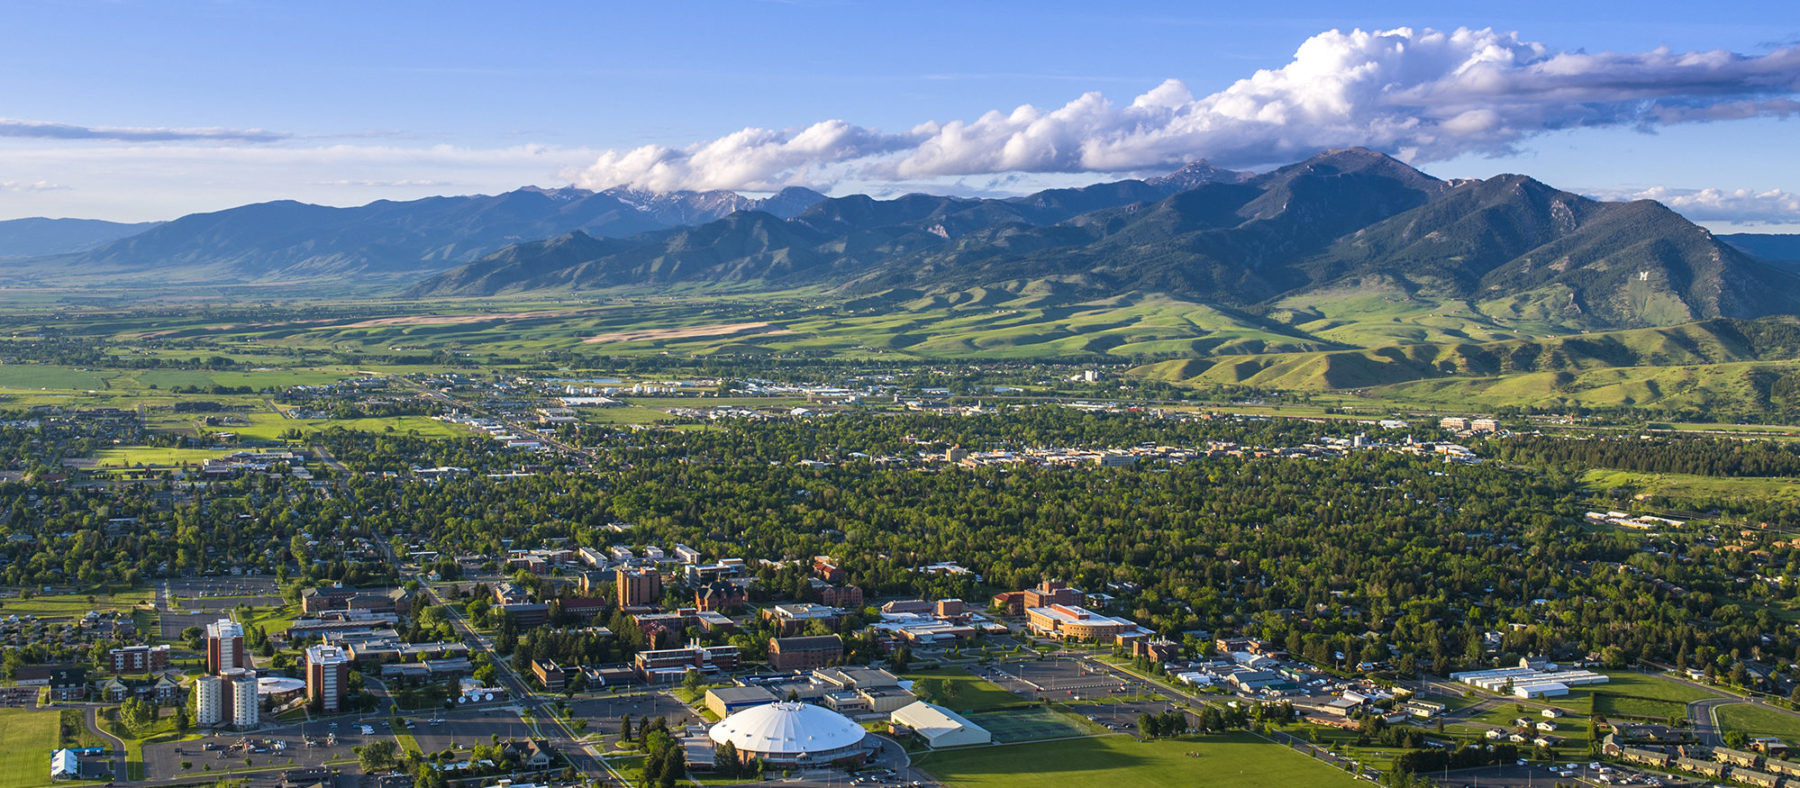
\includegraphics[width=5in,height=\textheight]{images/msu-campus.jpg}}
\usepackage{etoolbox}
\makeatletter
\providecommand{\subtitle}[1]{% add subtitle to \maketitle
  \apptocmd{\@title}{\par {\large #1 \par}}{}{}
}
\makeatother
\subtitle{Fall 2022\\
Montana State University}
\author{Melinda Yager\\
Jade Schmidt\\
Stacey Hancock}
\date{}

\begin{document}
\maketitle

\hypertarget{preface}{%
\chapter*{Preface}\label{preface}}
\addcontentsline{toc}{chapter}{Preface}

Placeholder

\hypertarget{fall-2022-calendar-of-in-class-activities}{%
\chapter*{Fall 2022 Calendar of In-Class Activities}\label{fall-2022-calendar-of-in-class-activities}}
\addcontentsline{toc}{chapter}{Fall 2022 Calendar of In-Class Activities}

Placeholder

\hypertarget{basics-of-data}{%
\chapter{Basics of Data}\label{basics-of-data}}

Placeholder

\hypertarget{week-1-reading-guide-basics-of-data}{%
\section{Week 1 Reading Guide: Basics of Data}\label{week-1-reading-guide-basics-of-data}}

\hypertarget{sections-1.1-case-study-and-1.2-data-basics}{%
\subsection*{Sections 1.1 (Case study) and 1.2 (Data basics)}\label{sections-1.1-case-study-and-1.2-data-basics}}
\addcontentsline{toc}{subsection}{Sections 1.1 (Case study) and 1.2 (Data basics)}

\hypertarget{vocabulary}{%
\subsubsection*{Vocabulary}\label{vocabulary}}
\addcontentsline{toc}{subsubsection}{Vocabulary}

\hypertarget{notes}{%
\subsubsection*{Notes}\label{notes}}
\addcontentsline{toc}{subsubsection}{Notes}

\hypertarget{example-section-1.1-case-study-using-stents-to-prevent-strokes}{%
\subsubsection*{Example (Section 1.1 --- Case study: Using stents to prevent strokes)}\label{example-section-1.1-case-study-using-stents-to-prevent-strokes}}
\addcontentsline{toc}{subsubsection}{Example (Section 1.1 --- Case study: Using stents to prevent strokes)}

\hypertarget{section-2.1-sampling-principles-and-strategies}{%
\subsection*{Section 2.1 (Sampling principles and strategies)}\label{section-2.1-sampling-principles-and-strategies}}
\addcontentsline{toc}{subsection}{Section 2.1 (Sampling principles and strategies)}

\hypertarget{vocabulary-1}{%
\subsubsection*{Vocabulary}\label{vocabulary-1}}
\addcontentsline{toc}{subsubsection}{Vocabulary}

\hypertarget{notes-1}{%
\subsubsection*{Notes}\label{notes-1}}
\addcontentsline{toc}{subsubsection}{Notes}

\hypertarget{notes-on-types-of-sampling-bias}{%
\paragraph*{Notes on types of sampling bias}\label{notes-on-types-of-sampling-bias}}
\addcontentsline{toc}{paragraph}{Notes on types of sampling bias}

\hypertarget{activity-1-intro-to-data}{%
\section{Activity 1: Intro to Data}\label{activity-1-intro-to-data}}

\hypertarget{learning-outcomes}{%
\subsection{Learning outcomes}\label{learning-outcomes}}

\hypertarget{terminology-review}{%
\subsection{Terminology review}\label{terminology-review}}

\hypertarget{general-information-on-the-coursepack}{%
\subsection{General information on the Coursepack}\label{general-information-on-the-coursepack}}

\hypertarget{general-information-on-labs}{%
\subsection{General information on labs}\label{general-information-on-labs}}

\hypertarget{steps-of-the-statistical-investigation-process}{%
\subsubsection*{Steps of the statistical investigation process}\label{steps-of-the-statistical-investigation-process}}
\addcontentsline{toc}{subsubsection}{Steps of the statistical investigation process}

\hypertarget{take-home-messages}{%
\subsection{Take-home messages}\label{take-home-messages}}

\hypertarget{additional-notes}{%
\subsection{Additional notes}\label{additional-notes}}

\hypertarget{study-design}{%
\chapter{Study Design}\label{study-design}}

Placeholder

\hypertarget{week-2-reading-guide-sampling-experimental-design-and-scope-of-inference}{%
\section{Week 2 Reading Guide: Sampling, Experimental Design, and Scope of Inference}\label{week-2-reading-guide-sampling-experimental-design-and-scope-of-inference}}

\hypertarget{sections-2.2-observational-studies-2.3-experiments-and-2.4-scope-of-inference}{%
\subsection*{Sections 2.2 (Observational studies), 2.3 (Experiments), and 2.4 (Scope of inference)}\label{sections-2.2-observational-studies-2.3-experiments-and-2.4-scope-of-inference}}
\addcontentsline{toc}{subsection}{Sections 2.2 (Observational studies), 2.3 (Experiments), and 2.4 (Scope of inference)}

\hypertarget{reminders-from-section-1.2}{%
\subsubsection*{Reminders from Section 1.2}\label{reminders-from-section-1.2}}
\addcontentsline{toc}{subsubsection}{Reminders from Section 1.2}

\hypertarget{vocabulary-2}{%
\subsubsection*{Vocabulary}\label{vocabulary-2}}
\addcontentsline{toc}{subsubsection}{Vocabulary}

\hypertarget{notes-2}{%
\subsubsection*{Notes}\label{notes-2}}
\addcontentsline{toc}{subsubsection}{Notes}

\hypertarget{activity-2a-american-indian-address}{%
\section{Activity 2A: American Indian Address}\label{activity-2a-american-indian-address}}

\hypertarget{learning-outcomes-1}{%
\subsection{Learning outcomes}\label{learning-outcomes-1}}

\hypertarget{terminology-review-1}{%
\subsection{Terminology review}\label{terminology-review-1}}

\hypertarget{american-indian-address}{%
\subsection{American Indian Address}\label{american-indian-address}}

\hypertarget{by-eye-selection}{%
\subsubsection*{By eye selection}\label{by-eye-selection}}
\addcontentsline{toc}{subsubsection}{By eye selection}

\hypertarget{take-home-messages-1}{%
\subsection{Take-home messages}\label{take-home-messages-1}}

\hypertarget{additional-notes-1}{%
\subsection{Additional notes}\label{additional-notes-1}}

\hypertarget{activity-2b-american-indian-address-continued}{%
\section{Activity 2B: American Indian Address (continued)}\label{activity-2b-american-indian-address-continued}}

\hypertarget{learning-outcomes-2}{%
\subsection{Learning outcomes}\label{learning-outcomes-2}}

\hypertarget{terminology-review-2}{%
\subsection{Terminology review}\label{terminology-review-2}}

\hypertarget{random-selection}{%
\subsubsection*{Random selection}\label{random-selection}}
\addcontentsline{toc}{subsubsection}{Random selection}

\hypertarget{effect-of-sample-size}{%
\subsection*{Effect of sample size}\label{effect-of-sample-size}}
\addcontentsline{toc}{subsection}{Effect of sample size}

\hypertarget{take-home-messages-2}{%
\subsection{Take-home messages}\label{take-home-messages-2}}

\hypertarget{additional-notes-2}{%
\subsection{Additional notes}\label{additional-notes-2}}

\hypertarget{week-2-lab-study-design}{%
\section{Week 2 Lab: Study Design}\label{week-2-lab-study-design}}

\hypertarget{learning-outcomes-3}{%
\subsection{Learning outcomes}\label{learning-outcomes-3}}

\hypertarget{terminology-review-3}{%
\subsection{Terminology review}\label{terminology-review-3}}

\hypertarget{general-information-labs}{%
\subsection{General information labs}\label{general-information-labs}}

\hypertarget{study-design-1}{%
\subsection*{Study design}\label{study-design-1}}
\addcontentsline{toc}{subsection}{Study design}

\hypertarget{atrial-fibrillation}{%
\subsection*{Atrial fibrillation}\label{atrial-fibrillation}}
\addcontentsline{toc}{subsection}{Atrial fibrillation}

\hypertarget{take-home-messages-3}{%
\subsection{Take-home messages}\label{take-home-messages-3}}

\hypertarget{additional-notes-3}{%
\subsection{Additional notes}\label{additional-notes-3}}

\hypertarget{exploring-categorical-and-quantitative-data}{%
\chapter{Exploring Categorical and Quantitative Data}\label{exploring-categorical-and-quantitative-data}}

Placeholder

\hypertarget{week-3-reading-guide-introduction-to-r-categorical-variables-and-a-single-quantitative-variable}{%
\section{Week 3 Reading Guide: Introduction to R, Categorical Variables, and a Single Quantitative Variable}\label{week-3-reading-guide-introduction-to-r-categorical-variables-and-a-single-quantitative-variable}}

\hypertarget{chapter-3-applications-data}{%
\subsection*{Chapter 3 (Applications: Data)}\label{chapter-3-applications-data}}
\addcontentsline{toc}{subsection}{Chapter 3 (Applications: Data)}

\hypertarget{notes-3}{%
\subsubsection*{Notes}\label{notes-3}}
\addcontentsline{toc}{subsubsection}{Notes}

\hypertarget{functions}{%
\subsubsection*{Functions}\label{functions}}
\addcontentsline{toc}{subsubsection}{Functions}

\hypertarget{chapter-4-exploring-categorical-data}{%
\subsection*{Chapter 4 (Exploring categorical data)}\label{chapter-4-exploring-categorical-data}}
\addcontentsline{toc}{subsection}{Chapter 4 (Exploring categorical data)}

\hypertarget{vocabulary-3}{%
\subsubsection*{Vocabulary}\label{vocabulary-3}}
\addcontentsline{toc}{subsubsection}{Vocabulary}

\hypertarget{notes-4}{%
\subsubsection*{Notes}\label{notes-4}}
\addcontentsline{toc}{subsubsection}{Notes}

\hypertarget{review-of-simpsons-paradox}{%
\subsubsection*{Review of Simpson's Paradox}\label{review-of-simpsons-paradox}}
\addcontentsline{toc}{subsubsection}{Review of Simpson's Paradox}

\hypertarget{chapter-5-exploring-quantitative-data}{%
\subsection*{Chapter 5 (Exploring quantitative data)}\label{chapter-5-exploring-quantitative-data}}
\addcontentsline{toc}{subsection}{Chapter 5 (Exploring quantitative data)}

\hypertarget{type-of-plots}{%
\subsubsection*{Type of Plots}\label{type-of-plots}}
\addcontentsline{toc}{subsubsection}{Type of Plots}

\hypertarget{vocabulary-4}{%
\subsubsection*{Vocabulary}\label{vocabulary-4}}
\addcontentsline{toc}{subsubsection}{Vocabulary}

\hypertarget{notes-5}{%
\subsubsection*{Notes}\label{notes-5}}
\addcontentsline{toc}{subsubsection}{Notes}

\hypertarget{summarizing-chapters-4-and-5}{%
\subsection{Summarizing Chapters 4 and 5}\label{summarizing-chapters-4-and-5}}

\hypertarget{notes-6}{%
\subsubsection*{Notes}\label{notes-6}}
\addcontentsline{toc}{subsubsection}{Notes}

\hypertarget{data-visualization-summary}{%
\subsubsection*{Data visualization summary}\label{data-visualization-summary}}
\addcontentsline{toc}{subsubsection}{Data visualization summary}

\hypertarget{activity-3-graphing-categorical-variables}{%
\section{Activity 3: Graphing Categorical Variables}\label{activity-3-graphing-categorical-variables}}

\hypertarget{learning-outcomes-4}{%
\subsection{Learning outcomes}\label{learning-outcomes-4}}

\hypertarget{terminology-review-4}{%
\subsection{Terminology review}\label{terminology-review-4}}

\hypertarget{graphing-categorical-variables}{%
\subsection{Graphing categorical variables}\label{graphing-categorical-variables}}

\hypertarget{nightlight-use-and-myopia}{%
\subsection*{Nightlight use and myopia}\label{nightlight-use-and-myopia}}
\addcontentsline{toc}{subsection}{Nightlight use and myopia}

\hypertarget{r-code}{%
\subsubsection*{R code}\label{r-code}}
\addcontentsline{toc}{subsubsection}{R code}

\hypertarget{displaying-a-single-categorical-variable}{%
\subsubsection*{Displaying a single categorical variable}\label{displaying-a-single-categorical-variable}}
\addcontentsline{toc}{subsubsection}{Displaying a single categorical variable}

\hypertarget{displaying-two-categorical-variables}{%
\subsubsection*{Displaying two categorical variables}\label{displaying-two-categorical-variables}}
\addcontentsline{toc}{subsubsection}{Displaying two categorical variables}

\hypertarget{take-home-messages-4}{%
\subsection{Take-home messages}\label{take-home-messages-4}}

\hypertarget{additional-notes-4}{%
\subsection{Additional notes}\label{additional-notes-4}}

\hypertarget{week-3-lab-ipeds}{%
\section{Week 3 Lab: IPEDs}\label{week-3-lab-ipeds}}

\hypertarget{learning-outcomes-5}{%
\subsection{Learning outcomes}\label{learning-outcomes-5}}

\hypertarget{terminology-review-5}{%
\subsection{Terminology review}\label{terminology-review-5}}

\hypertarget{the-integrated-postsecondary-education-data-system-ipeds}{%
\subsection{The Integrated Postsecondary Education Data System (IPEDS)}\label{the-integrated-postsecondary-education-data-system-ipeds}}

\hypertarget{summary-statistics-for-a-single-quantitative-variable}{%
\subsubsection*{Summary statistics for a single quantitative variable}\label{summary-statistics-for-a-single-quantitative-variable}}
\addcontentsline{toc}{subsubsection}{Summary statistics for a single quantitative variable}

\hypertarget{displaying-a-single-quantitative-variable}{%
\subsubsection*{Displaying a single quantitative variable}\label{displaying-a-single-quantitative-variable}}
\addcontentsline{toc}{subsubsection}{Displaying a single quantitative variable}

\hypertarget{robust-statistics}{%
\subsubsection*{Robust Statistics}\label{robust-statistics}}
\addcontentsline{toc}{subsubsection}{Robust Statistics}

\hypertarget{summarizing-a-single-categorical-and-single-quantitative-variable}{%
\subsubsection*{Summarizing a single categorical and single quantitative variable}\label{summarizing-a-single-categorical-and-single-quantitative-variable}}
\addcontentsline{toc}{subsubsection}{Summarizing a single categorical and single quantitative variable}

\hypertarget{take-home-messages-5}{%
\subsection{Take-home messages}\label{take-home-messages-5}}

\hypertarget{exploring-multivariable-data}{%
\chapter{Exploring Multivariable Data}\label{exploring-multivariable-data}}

Placeholder

\hypertarget{week-4-reading-guide-two-quantitative-variables-and-multivariable-concepts}{%
\section{Week 4 Reading Guide: Two Quantitative Variables and Multivariable Concepts}\label{week-4-reading-guide-two-quantitative-variables-and-multivariable-concepts}}

\hypertarget{section-6.1-fitting-a-line-residuals-and-correlation}{%
\subsection*{Section 6.1 (Fitting a line, residuals, and correlation)}\label{section-6.1-fitting-a-line-residuals-and-correlation}}
\addcontentsline{toc}{subsection}{Section 6.1 (Fitting a line, residuals, and correlation)}

\hypertarget{reminders-from-section-5.1}{%
\subsubsection*{Reminders from Section 5.1}\label{reminders-from-section-5.1}}
\addcontentsline{toc}{subsubsection}{Reminders from Section 5.1}

\hypertarget{vocabulary-5}{%
\subsubsection*{Vocabulary}\label{vocabulary-5}}
\addcontentsline{toc}{subsubsection}{Vocabulary}

\hypertarget{notes-7}{%
\subsubsection*{Notes}\label{notes-7}}
\addcontentsline{toc}{subsubsection}{Notes}

\hypertarget{example-brushtail-possums}{%
\subsubsection*{Example: Brushtail possums}\label{example-brushtail-possums}}
\addcontentsline{toc}{subsubsection}{Example: Brushtail possums}

\hypertarget{section-6.2-least-squares-regression}{%
\subsection*{Section 6.2 (Least squares regression)}\label{section-6.2-least-squares-regression}}
\addcontentsline{toc}{subsection}{Section 6.2 (Least squares regression)}

\hypertarget{vocabulary-6}{%
\subsubsection*{Vocabulary}\label{vocabulary-6}}
\addcontentsline{toc}{subsubsection}{Vocabulary}

\hypertarget{notes-8}{%
\subsubsection*{Notes}\label{notes-8}}
\addcontentsline{toc}{subsubsection}{Notes}

\hypertarget{example-elmhurst-college}{%
\subsubsection*{Example: Elmhurst College}\label{example-elmhurst-college}}
\addcontentsline{toc}{subsubsection}{Example: Elmhurst College}

\hypertarget{section-6.3-outliers-in-linear-regression}{%
\subsection*{Section 6.3 (Outliers in linear regression)}\label{section-6.3-outliers-in-linear-regression}}
\addcontentsline{toc}{subsection}{Section 6.3 (Outliers in linear regression)}

\hypertarget{vocabulary-7}{%
\subsubsection*{Vocabulary}\label{vocabulary-7}}
\addcontentsline{toc}{subsubsection}{Vocabulary}

\hypertarget{notes-9}{%
\subsubsection*{Notes}\label{notes-9}}
\addcontentsline{toc}{subsubsection}{Notes}

\hypertarget{section-6.4-chapter-6-review}{%
\subsection*{Section 6.4 (Chapter 6 review)}\label{section-6.4-chapter-6-review}}
\addcontentsline{toc}{subsection}{Section 6.4 (Chapter 6 review)}

\hypertarget{notes-10}{%
\subsubsection*{Notes}\label{notes-10}}
\addcontentsline{toc}{subsubsection}{Notes}

\hypertarget{section-7.1-gapminder-world}{%
\subsection*{Section 7.1 (Gapminder world)}\label{section-7.1-gapminder-world}}
\addcontentsline{toc}{subsection}{Section 7.1 (Gapminder world)}

\hypertarget{vocabulary-8}{%
\subsubsection*{Vocabulary}\label{vocabulary-8}}
\addcontentsline{toc}{subsubsection}{Vocabulary}

\hypertarget{notes-11}{%
\subsubsection*{Notes}\label{notes-11}}
\addcontentsline{toc}{subsubsection}{Notes}

\hypertarget{section-7.2-simpsons-paradox-revisited}{%
\subsection*{Section 7.2 (Simpson's Paradox, revisited)}\label{section-7.2-simpsons-paradox-revisited}}
\addcontentsline{toc}{subsection}{Section 7.2 (Simpson's Paradox, revisited)}

\hypertarget{reminder-from-section-4.4}{%
\subsubsection*{Reminder from Section 4.4}\label{reminder-from-section-4.4}}
\addcontentsline{toc}{subsubsection}{Reminder from Section 4.4}

\hypertarget{notes-12}{%
\subsubsection*{Notes}\label{notes-12}}
\addcontentsline{toc}{subsubsection}{Notes}

\hypertarget{example-sat-scores}{%
\subsubsection*{Example: SAT scores}\label{example-sat-scores}}
\addcontentsline{toc}{subsubsection}{Example: SAT scores}

\hypertarget{activity-4a-movie-profits-linear-regression}{%
\section{Activity 4A: Movie Profits --- Linear Regression}\label{activity-4a-movie-profits-linear-regression}}

\hypertarget{learning-outcomes-6}{%
\subsection{Learning outcomes}\label{learning-outcomes-6}}

\hypertarget{terminology-review-6}{%
\subsection{Terminology review}\label{terminology-review-6}}

\hypertarget{movies-released-in-2016}{%
\subsection{Movies released in 2016}\label{movies-released-in-2016}}

\hypertarget{vocabulary-review}{%
\subsubsection*{Vocabulary review}\label{vocabulary-review}}
\addcontentsline{toc}{subsubsection}{Vocabulary review}

\hypertarget{slope}{%
\subsubsection*{Slope}\label{slope}}
\addcontentsline{toc}{subsubsection}{Slope}

\hypertarget{residuals}{%
\subsubsection*{Residuals}\label{residuals}}
\addcontentsline{toc}{subsubsection}{Residuals}

\hypertarget{multivariable-plots}{%
\subsubsection*{Multivariable plots}\label{multivariable-plots}}
\addcontentsline{toc}{subsubsection}{Multivariable plots}

\hypertarget{take-home-messages-6}{%
\subsection{Take-home messages}\label{take-home-messages-6}}

\hypertarget{additional-notes-5}{%
\subsection{Additional notes}\label{additional-notes-5}}

\hypertarget{activity-4b-movie-profits-correlation-and-coefficient-of-determination}{%
\section{Activity 4B: Movie Profits --- Correlation and Coefficient of Determination}\label{activity-4b-movie-profits-correlation-and-coefficient-of-determination}}

\hypertarget{learning-outcomes-7}{%
\subsection{Learning outcomes}\label{learning-outcomes-7}}

\hypertarget{terminology-review-7}{%
\subsection{Terminology review}\label{terminology-review-7}}

\hypertarget{movies-released-in-2016-1}{%
\subsection{Movies released in 2016}\label{movies-released-in-2016-1}}

\hypertarget{correlation}{%
\subsubsection*{Correlation}\label{correlation}}
\addcontentsline{toc}{subsubsection}{Correlation}

\hypertarget{coefficient-of-determination-squared-correlation}{%
\subsubsection*{Coefficient of determination (squared correlation)}\label{coefficient-of-determination-squared-correlation}}
\addcontentsline{toc}{subsubsection}{Coefficient of determination (squared correlation)}

\hypertarget{take-home-messages-7}{%
\subsection{Take-home messages}\label{take-home-messages-7}}

\hypertarget{additional-notes-6}{%
\subsection{Additional notes}\label{additional-notes-6}}

\hypertarget{week-4-lab-penguins}{%
\section{Week 4 Lab: Penguins}\label{week-4-lab-penguins}}

\hypertarget{learning-outcomes-8}{%
\subsection{Learning outcomes}\label{learning-outcomes-8}}

\hypertarget{penguins}{%
\subsection{Penguins}\label{penguins}}

\hypertarget{exam-1-review}{%
\chapter{Exam 1 Review}\label{exam-1-review}}

Placeholder

\hypertarget{inference-for-a-single-categorical-variable-simulation-based-methods}{%
\chapter{Inference for a Single Categorical Variable: Simulation-based Methods}\label{inference-for-a-single-categorical-variable-simulation-based-methods}}

Placeholder

\hypertarget{week-6-reading-guide-categorical-inference}{%
\section{Week 6 Reading Guide: Categorical Inference}\label{week-6-reading-guide-categorical-inference}}

\hypertarget{chapter-9-hypothesis-testing-with-randomization}{%
\subsection*{Chapter 9 (Hypothesis testing with randomization)}\label{chapter-9-hypothesis-testing-with-randomization}}
\addcontentsline{toc}{subsection}{Chapter 9 (Hypothesis testing with randomization)}

\hypertarget{reminders-from-previous-sections}{%
\subsubsection*{Reminders from previous sections}\label{reminders-from-previous-sections}}
\addcontentsline{toc}{subsubsection}{Reminders from previous sections}

\hypertarget{vocabulary-9}{%
\subsubsection*{Vocabulary}\label{vocabulary-9}}
\addcontentsline{toc}{subsubsection}{Vocabulary}

\hypertarget{notes-13}{%
\subsubsection*{Notes}\label{notes-13}}
\addcontentsline{toc}{subsubsection}{Notes}

\hypertarget{example-from-section-9.1-martian-alphabet}{%
\subsubsection*{Example from section 9.1: Martian alphabet}\label{example-from-section-9.1-martian-alphabet}}
\addcontentsline{toc}{subsubsection}{Example from section 9.1: Martian alphabet}

\hypertarget{example-from-section-9.2-sex-discrimination}{%
\subsubsection*{Example from section 9.2: Sex discrimination}\label{example-from-section-9.2-sex-discrimination}}
\addcontentsline{toc}{subsubsection}{Example from section 9.2: Sex discrimination}

\hypertarget{chapter-10-confidence-intervals-with-bootstrapping}{%
\subsection*{Chapter 10 (Confidence intervals with bootstrapping)}\label{chapter-10-confidence-intervals-with-bootstrapping}}
\addcontentsline{toc}{subsection}{Chapter 10 (Confidence intervals with bootstrapping)}

\hypertarget{reminders-from-previous-sections-1}{%
\subsubsection*{Reminders from previous sections}\label{reminders-from-previous-sections-1}}
\addcontentsline{toc}{subsubsection}{Reminders from previous sections}

\hypertarget{vocabulary-10}{%
\subsubsection*{Vocabulary}\label{vocabulary-10}}
\addcontentsline{toc}{subsubsection}{Vocabulary}

\hypertarget{notes-14}{%
\subsubsection*{Notes}\label{notes-14}}
\addcontentsline{toc}{subsubsection}{Notes}

\hypertarget{example-medical-consultant}{%
\subsubsection*{Example: Medical consultant}\label{example-medical-consultant}}
\addcontentsline{toc}{subsubsection}{Example: Medical consultant}

\hypertarget{section-14.1-simulation-based-test-for-h_0pi-pi_0}{%
\subsection*{\texorpdfstring{Section 14.1 (Simulation-based test for \(H_0:\pi = \pi_0\))}{Section 14.1 (Simulation-based test for H\_0:\textbackslash pi = \textbackslash pi\_0)}}\label{section-14.1-simulation-based-test-for-h_0pi-pi_0}}
\addcontentsline{toc}{subsection}{Section 14.1 (Simulation-based test for \(H_0:\pi = \pi_0\))}

\hypertarget{reminders-from-previous-sections-2}{%
\subsubsection*{Reminders from previous sections}\label{reminders-from-previous-sections-2}}
\addcontentsline{toc}{subsubsection}{Reminders from previous sections}

\hypertarget{vocabulary-11}{%
\subsubsection*{Vocabulary}\label{vocabulary-11}}
\addcontentsline{toc}{subsubsection}{Vocabulary}

\hypertarget{notes-15}{%
\subsubsection*{Notes}\label{notes-15}}
\addcontentsline{toc}{subsubsection}{Notes}

\hypertarget{example-medical-consultant-1}{%
\subsubsection*{Example: Medical consultant}\label{example-medical-consultant-1}}
\addcontentsline{toc}{subsubsection}{Example: Medical consultant}

\hypertarget{section-14.2-bootstrap-confidence-interval-for-pi}{%
\subsection*{\texorpdfstring{Section 14.2 (Bootstrap confidence interval for \(\pi\))}{Section 14.2 (Bootstrap confidence interval for \textbackslash pi)}}\label{section-14.2-bootstrap-confidence-interval-for-pi}}
\addcontentsline{toc}{subsection}{Section 14.2 (Bootstrap confidence interval for \(\pi\))}

\hypertarget{reminders-from-previous-sections-3}{%
\subsubsection*{Reminders from previous sections}\label{reminders-from-previous-sections-3}}
\addcontentsline{toc}{subsubsection}{Reminders from previous sections}

\hypertarget{notes-16}{%
\subsubsection*{Notes}\label{notes-16}}
\addcontentsline{toc}{subsubsection}{Notes}

\hypertarget{example-medical-consultant-2}{%
\subsubsection*{Example: Medical consultant}\label{example-medical-consultant-2}}
\addcontentsline{toc}{subsubsection}{Example: Medical consultant}

\hypertarget{activity-6a-helperer-hinderer-simulation-based-hypothesis-test}{%
\section{Activity 6A: Helperer-Hinderer --- Simulation-based Hypothesis Test}\label{activity-6a-helperer-hinderer-simulation-based-hypothesis-test}}

\hypertarget{learning-outcomes-9}{%
\subsection{Learning outcomes}\label{learning-outcomes-9}}

\hypertarget{terminology-review-8}{%
\subsection{Terminology review}\label{terminology-review-8}}

\hypertarget{steps-of-the-statistical-investigation-process-1}{%
\subsection{Steps of the statistical investigation process}\label{steps-of-the-statistical-investigation-process-1}}

\hypertarget{helper-hinderer}{%
\subsection{Helper-Hinderer}\label{helper-hinderer}}

\hypertarget{ask-a-research-question}{%
\subsubsection*{Ask a research question}\label{ask-a-research-question}}
\addcontentsline{toc}{subsubsection}{Ask a research question}

\hypertarget{design-a-study-and-collect-data}{%
\subsubsection*{Design a study and collect data}\label{design-a-study-and-collect-data}}
\addcontentsline{toc}{subsubsection}{Design a study and collect data}

\hypertarget{summarize-and-visualize-the-data}{%
\subsubsection*{Summarize and visualize the data}\label{summarize-and-visualize-the-data}}
\addcontentsline{toc}{subsubsection}{Summarize and visualize the data}

\hypertarget{use-statistical-analysis-methods-to-draw-inferences-from-the-data}{%
\subsubsection*{Use statistical analysis methods to draw inferences from the data}\label{use-statistical-analysis-methods-to-draw-inferences-from-the-data}}
\addcontentsline{toc}{subsubsection}{Use statistical analysis methods to draw inferences from the data}

\hypertarget{take-home-messages-8}{%
\subsection{Take-home messages}\label{take-home-messages-8}}

\hypertarget{additional-notes-7}{%
\subsection{Additional notes}\label{additional-notes-7}}

\hypertarget{activity-6b-helper-hinderer-continued}{%
\section{Activity 6B: Helper-Hinderer (continued)}\label{activity-6b-helper-hinderer-continued}}

\hypertarget{learning-outcomes-10}{%
\subsection{Learning outcomes}\label{learning-outcomes-10}}

\hypertarget{steps-of-the-statistical-investigation-process-2}{%
\subsection{Steps of the statistical investigation process}\label{steps-of-the-statistical-investigation-process-2}}

\hypertarget{helper-hinderer-1}{%
\subsection{Helper-Hinderer}\label{helper-hinderer-1}}

\hypertarget{interpret-the-p-value}{%
\subsubsection*{Interpret the p-value}\label{interpret-the-p-value}}
\addcontentsline{toc}{subsubsection}{Interpret the p-value}

\hypertarget{communicate-the-results-and-answer-the-research-question}{%
\subsubsection*{Communicate the results and answer the research question}\label{communicate-the-results-and-answer-the-research-question}}
\addcontentsline{toc}{subsubsection}{Communicate the results and answer the research question}

\hypertarget{take-home-messages-9}{%
\subsection{Take-home messages}\label{take-home-messages-9}}

\hypertarget{additional-notes-8}{%
\subsection{Additional notes}\label{additional-notes-8}}

\hypertarget{week-6-lab-helper-hinderer-simulation-based-confidence-interval}{%
\section{Week 6 Lab: Helper-Hinderer --- Simulation-based Confidence Interval}\label{week-6-lab-helper-hinderer-simulation-based-confidence-interval}}

\hypertarget{learning-outcomes-11}{%
\subsection{Learning outcomes}\label{learning-outcomes-11}}

\hypertarget{terminology-review-9}{%
\subsection{Terminology review}\label{terminology-review-9}}

\hypertarget{helper-hinderer-2}{%
\subsection{Helper-Hinderer}\label{helper-hinderer-2}}

\hypertarget{activity-intro}{%
\subsubsection*{Activity intro}\label{activity-intro}}
\addcontentsline{toc}{subsubsection}{Activity intro}

\hypertarget{use-statistical-analysis-methods-to-draw-inferences-from-the-data-1}{%
\subsubsection*{Use statistical analysis methods to draw inferences from the data}\label{use-statistical-analysis-methods-to-draw-inferences-from-the-data-1}}
\addcontentsline{toc}{subsubsection}{Use statistical analysis methods to draw inferences from the data}

\hypertarget{communicate-the-results-and-answer-the-research-question-1}{%
\subsubsection*{Communicate the results and answer the research question}\label{communicate-the-results-and-answer-the-research-question-1}}
\addcontentsline{toc}{subsubsection}{Communicate the results and answer the research question}

\hypertarget{effect-of-confidence-level}{%
\subsubsection*{Effect of confidence level}\label{effect-of-confidence-level}}
\addcontentsline{toc}{subsubsection}{Effect of confidence level}

\hypertarget{take-home-messages-10}{%
\subsection{Take-home messages}\label{take-home-messages-10}}

\hypertarget{additional-notes-9}{%
\subsection{Additional notes}\label{additional-notes-9}}

\hypertarget{inference-for-a-single-categorical-variable-theory-based-methods-errors-and-power}{%
\chapter{Inference for a Single Categorical Variable: Theory-based Methods + Errors and Power}\label{inference-for-a-single-categorical-variable-theory-based-methods-errors-and-power}}

Placeholder

\hypertarget{week-7-reading-guide-categorical-inference}{%
\section{Week 7 Reading Guide: Categorical Inference}\label{week-7-reading-guide-categorical-inference}}

\hypertarget{chapter-11-inference-with-mathematical-models}{%
\subsection*{Chapter 11 (Inference with mathematical models)}\label{chapter-11-inference-with-mathematical-models}}
\addcontentsline{toc}{subsection}{Chapter 11 (Inference with mathematical models)}

\hypertarget{reminders-from-previous-sections-4}{%
\subsubsection*{Reminders from previous sections}\label{reminders-from-previous-sections-4}}
\addcontentsline{toc}{subsubsection}{Reminders from previous sections}

\hypertarget{vocabulary-12}{%
\subsubsection*{Vocabulary}\label{vocabulary-12}}
\addcontentsline{toc}{subsubsection}{Vocabulary}

\hypertarget{notes-17}{%
\subsubsection*{Notes}\label{notes-17}}
\addcontentsline{toc}{subsubsection}{Notes}

\hypertarget{formulas}{%
\subsubsection*{Formulas}\label{formulas}}
\addcontentsline{toc}{subsubsection}{Formulas}

\hypertarget{r-coding}{%
\subsection*{R coding}\label{r-coding}}
\addcontentsline{toc}{subsection}{R coding}

\hypertarget{calculating-normal-probabilities}{%
\paragraph*{Calculating normal probabilities}\label{calculating-normal-probabilities}}
\addcontentsline{toc}{paragraph}{Calculating normal probabilities}

\hypertarget{displaying-normal-probabilities}{%
\paragraph*{Displaying normal probabilities}\label{displaying-normal-probabilities}}
\addcontentsline{toc}{paragraph}{Displaying normal probabilities}

\hypertarget{calculating-normal-percentiles}{%
\paragraph*{Calculating normal percentiles}\label{calculating-normal-percentiles}}
\addcontentsline{toc}{paragraph}{Calculating normal percentiles}

\hypertarget{section-14.3-theory-based-inferential-methods-for-pi}{%
\subsection*{\texorpdfstring{Section 14.3 (Theory-based inferential methods for \(\pi\))}{Section 14.3 (Theory-based inferential methods for \textbackslash pi)}}\label{section-14.3-theory-based-inferential-methods-for-pi}}
\addcontentsline{toc}{subsection}{Section 14.3 (Theory-based inferential methods for \(\pi\))}

\hypertarget{vocabulary-13}{%
\subsubsection*{Vocabulary}\label{vocabulary-13}}
\addcontentsline{toc}{subsubsection}{Vocabulary}

\hypertarget{reminders-from-previous-sections-5}{%
\subsubsection*{Reminders from previous sections}\label{reminders-from-previous-sections-5}}
\addcontentsline{toc}{subsubsection}{Reminders from previous sections}

\hypertarget{vocabulary-14}{%
\subsubsection*{Vocabulary}\label{vocabulary-14}}
\addcontentsline{toc}{subsubsection}{Vocabulary}

\hypertarget{notes-18}{%
\subsubsection*{Notes}\label{notes-18}}
\addcontentsline{toc}{subsubsection}{Notes}

\hypertarget{formulas-1}{%
\subsubsection*{Formulas}\label{formulas-1}}
\addcontentsline{toc}{subsubsection}{Formulas}

\hypertarget{example-payday-loans}{%
\subsubsection*{Example: Payday loans}\label{example-payday-loans}}
\addcontentsline{toc}{subsubsection}{Example: Payday loans}

\hypertarget{chapter-12-errors-power-and-practical-importance}{%
\subsection*{Chapter 12 (Errors, power, and practical importance)}\label{chapter-12-errors-power-and-practical-importance}}
\addcontentsline{toc}{subsection}{Chapter 12 (Errors, power, and practical importance)}

\hypertarget{reminders-from-previous-sections-6}{%
\subsubsection*{Reminders from previous sections}\label{reminders-from-previous-sections-6}}
\addcontentsline{toc}{subsubsection}{Reminders from previous sections}

\hypertarget{vocabulary-15}{%
\subsubsection*{Vocabulary}\label{vocabulary-15}}
\addcontentsline{toc}{subsubsection}{Vocabulary}

\hypertarget{notes-19}{%
\subsubsection*{Notes}\label{notes-19}}
\addcontentsline{toc}{subsubsection}{Notes}

\hypertarget{examples}{%
\subsubsection*{Examples:}\label{examples}}
\addcontentsline{toc}{subsubsection}{Examples:}

\hypertarget{activity-7a-handedness-of-male-boxers-theory-based-hypothesis-test}{%
\section{Activity 7A: Handedness of Male Boxers --- Theory-based Hypothesis Test}\label{activity-7a-handedness-of-male-boxers-theory-based-hypothesis-test}}

\hypertarget{learning-outcomes-12}{%
\subsection{Learning outcomes}\label{learning-outcomes-12}}

\hypertarget{terminology-review-10}{%
\subsection{Terminology review}\label{terminology-review-10}}

\hypertarget{handedness-of-male-boxers}{%
\subsection{Handedness of male boxers}\label{handedness-of-male-boxers}}

\hypertarget{review-of-summary-statistics}{%
\subsection*{Review of summary statistics}\label{review-of-summary-statistics}}
\addcontentsline{toc}{subsection}{Review of summary statistics}

\hypertarget{theory-based-methods}{%
\subsection*{Theory-based methods}\label{theory-based-methods}}
\addcontentsline{toc}{subsection}{Theory-based methods}

\hypertarget{impacts-on-the-p-value}{%
\subsection*{Impacts on the P-value}\label{impacts-on-the-p-value}}
\addcontentsline{toc}{subsection}{Impacts on the P-value}

\hypertarget{take-home-messages-11}{%
\subsection{Take-home messages}\label{take-home-messages-11}}

\hypertarget{additional-notes-10}{%
\subsection{Additional notes}\label{additional-notes-10}}

\hypertarget{activity-7b-handedness-of-male-boxers-theory-based-confidence-interval}{%
\section{Activity 7B: Handedness of Male Boxers --- Theory-based Confidence Interval}\label{activity-7b-handedness-of-male-boxers-theory-based-confidence-interval}}

\hypertarget{learning-objectives}{%
\subsection{Learning objectives}\label{learning-objectives}}

\hypertarget{terminology-review-11}{%
\subsection{Terminology review}\label{terminology-review-11}}

\hypertarget{handedness-of-male-boxers-1}{%
\subsection{Handedness of Male Boxers}\label{handedness-of-male-boxers-1}}

\hypertarget{theory-based-confidence-interval}{%
\subsubsection*{Theory-based confidence interval}\label{theory-based-confidence-interval}}
\addcontentsline{toc}{subsubsection}{Theory-based confidence interval}

\hypertarget{simulation-methods}{%
\subsubsection*{Simulation Methods}\label{simulation-methods}}
\addcontentsline{toc}{subsubsection}{Simulation Methods}

\hypertarget{what-does-confidence-mean}{%
\subsection*{\texorpdfstring{What does \emph{confidence} mean?}{What does confidence mean?}}\label{what-does-confidence-mean}}
\addcontentsline{toc}{subsection}{What does \emph{confidence} mean?}

\hypertarget{take-home-messages-12}{%
\subsection{Take-home messages}\label{take-home-messages-12}}

\hypertarget{additional-notes-11}{%
\subsection{Additional notes}\label{additional-notes-11}}

\hypertarget{week-7-lab-errors-and-power}{%
\section{Week 7 Lab: Errors and Power}\label{week-7-lab-errors-and-power}}

\hypertarget{learning-outcomes-13}{%
\subsection{Learning outcomes}\label{learning-outcomes-13}}

\hypertarget{terminology-review-12}{%
\subsection{Terminology review}\label{terminology-review-12}}

\hypertarget{acl-recovery}{%
\subsection{ACL recovery}\label{acl-recovery}}

\hypertarget{inference-for-two-categorical-variables-simulation-based-methods}{%
\chapter{Inference for Two Categorical Variables: Simulation-based Methods}\label{inference-for-two-categorical-variables-simulation-based-methods}}

Placeholder

\hypertarget{week-8-reading-guide-hypothesis-testing-for-a-difference-in-proportions}{%
\section{Week 8 Reading Guide: Hypothesis Testing for a Difference in Proportions}\label{week-8-reading-guide-hypothesis-testing-for-a-difference-in-proportions}}

\hypertarget{section-15.1-randomization-test-for-h_0-pi_1---pi_2-0-and-section-15.2-bootstrap-confidence-interval-for-pi_1---pi_2}{%
\subsection*{\texorpdfstring{Section 15.1 (Randomization test for \(H_0: \pi_1 - \pi_2 = 0\)) and Section 15.2 (Bootstrap confidence interval for \(\pi_1 - \pi_2\))}{Section 15.1 (Randomization test for H\_0: \textbackslash pi\_1 - \textbackslash pi\_2 = 0) and Section 15.2 (Bootstrap confidence interval for \textbackslash pi\_1 - \textbackslash pi\_2)}}\label{section-15.1-randomization-test-for-h_0-pi_1---pi_2-0-and-section-15.2-bootstrap-confidence-interval-for-pi_1---pi_2}}
\addcontentsline{toc}{subsection}{Section 15.1 (Randomization test for \(H_0: \pi_1 - \pi_2 = 0\)) and Section 15.2 (Bootstrap confidence interval for \(\pi_1 - \pi_2\))}

\hypertarget{reminders-from-previous-sections-7}{%
\subsubsection*{Reminders from previous sections}\label{reminders-from-previous-sections-7}}
\addcontentsline{toc}{subsubsection}{Reminders from previous sections}

\hypertarget{vocabulary-16}{%
\subsubsection*{Vocabulary}\label{vocabulary-16}}
\addcontentsline{toc}{subsubsection}{Vocabulary}

\hypertarget{notes-20}{%
\subsubsection*{Notes}\label{notes-20}}
\addcontentsline{toc}{subsubsection}{Notes}

\hypertarget{notation}{%
\subsubsection*{Notation}\label{notation}}
\addcontentsline{toc}{subsubsection}{Notation}

\hypertarget{example-gender-discrimination}{%
\subsubsection*{Example: Gender discrimination}\label{example-gender-discrimination}}
\addcontentsline{toc}{subsubsection}{Example: Gender discrimination}

\hypertarget{example-opportunity-cost}{%
\subsubsection*{Example: Opportunity cost}\label{example-opportunity-cost}}
\addcontentsline{toc}{subsubsection}{Example: Opportunity cost}

\hypertarget{example-cpr-and-blood-thinners}{%
\subsubsection*{Example: CPR and blood thinners}\label{example-cpr-and-blood-thinners}}
\addcontentsline{toc}{subsubsection}{Example: CPR and blood thinners}

\hypertarget{activity-8a-the-good-samaritan-simulation-based-hypothesis-test}{%
\section{Activity 8A: The Good Samaritan --- Simulation-based Hypothesis Test}\label{activity-8a-the-good-samaritan-simulation-based-hypothesis-test}}

\hypertarget{learning-outcomes-14}{%
\subsection{Learning outcomes}\label{learning-outcomes-14}}

\hypertarget{terminology-review-13}{%
\subsection{Terminology review}\label{terminology-review-13}}

\hypertarget{the-good-samaritan}{%
\subsection{The Good Samaritan}\label{the-good-samaritan}}

\hypertarget{vocabulary-review-1}{%
\subsubsection*{Vocabulary review}\label{vocabulary-review-1}}
\addcontentsline{toc}{subsubsection}{Vocabulary review}

\hypertarget{ask-a-research-question-1}{%
\subsubsection*{Ask a research question}\label{ask-a-research-question-1}}
\addcontentsline{toc}{subsubsection}{Ask a research question}

\hypertarget{summarize-and-visualize-the-data-1}{%
\subsubsection*{Summarize and visualize the data}\label{summarize-and-visualize-the-data-1}}
\addcontentsline{toc}{subsubsection}{Summarize and visualize the data}

\hypertarget{take-home-messages-13}{%
\subsection{Take-home messages}\label{take-home-messages-13}}

\hypertarget{additional-notes-12}{%
\subsection{Additional notes}\label{additional-notes-12}}

\hypertarget{activity-8b-the-good-samaritan-continued-simulation-based-confidence-interval}{%
\section{Activity 8B: The Good Samaritan (continued) --- Simulation-based Confidence Interval}\label{activity-8b-the-good-samaritan-continued-simulation-based-confidence-interval}}

\hypertarget{learning-outcomes-15}{%
\subsection{Learning outcomes}\label{learning-outcomes-15}}

\hypertarget{terminology-review-14}{%
\subsection{Terminology review}\label{terminology-review-14}}

\hypertarget{the-good-samaritan-1}{%
\subsection{The Good Samaritan}\label{the-good-samaritan-1}}

\hypertarget{vocabulary-review-2}{%
\subsubsection*{Vocabulary review}\label{vocabulary-review-2}}
\addcontentsline{toc}{subsubsection}{Vocabulary review}

\hypertarget{use-statistical-analysis-methods-to-draw-inferences-from-the-data-2}{%
\subsubsection*{Use statistical analysis methods to draw inferences from the data}\label{use-statistical-analysis-methods-to-draw-inferences-from-the-data-2}}
\addcontentsline{toc}{subsubsection}{Use statistical analysis methods to draw inferences from the data}

\hypertarget{types-of-errors}{%
\subsubsection*{Types of errors}\label{types-of-errors}}
\addcontentsline{toc}{subsubsection}{Types of errors}

\hypertarget{take-home-messages-14}{%
\subsection{Take-home messages}\label{take-home-messages-14}}

\hypertarget{additional-notes-13}{%
\subsection{Additional notes}\label{additional-notes-13}}

\hypertarget{week-8-lab-poisonous-mushrooms}{%
\section{Week 8 Lab: Poisonous Mushrooms}\label{week-8-lab-poisonous-mushrooms}}

\hypertarget{learning-outcomes-16}{%
\subsection{Learning outcomes}\label{learning-outcomes-16}}

\hypertarget{poisonous-mushrooms}{%
\subsection{Poisonous Mushrooms}\label{poisonous-mushrooms}}

\hypertarget{inference-for-two-categorical-variables-theory-based-methods}{%
\chapter{Inference for Two Categorical Variables: Theory-based Methods}\label{inference-for-two-categorical-variables-theory-based-methods}}

Placeholder

\hypertarget{week-9-reading-guide-theory-based-inference-for-a-difference-in-proportions}{%
\section{Week 9 Reading Guide: Theory-based Inference for a Difference in Proportions}\label{week-9-reading-guide-theory-based-inference-for-a-difference-in-proportions}}

\hypertarget{section-15.3-theory-based-inferential-methods-for-pi_1---pi_2}{%
\subsection{\texorpdfstring{Section 15.3 (Theory-based inferential methods for \(\pi_1 - \pi_2\))}{Section 15.3 (Theory-based inferential methods for \textbackslash pi\_1 - \textbackslash pi\_2)}}\label{section-15.3-theory-based-inferential-methods-for-pi_1---pi_2}}

\hypertarget{reminders-from-previous-sections-8}{%
\subsubsection*{Reminders from previous sections}\label{reminders-from-previous-sections-8}}
\addcontentsline{toc}{subsubsection}{Reminders from previous sections}

\hypertarget{notes-21}{%
\subsubsection*{Notes}\label{notes-21}}
\addcontentsline{toc}{subsubsection}{Notes}

\hypertarget{formulas-2}{%
\subsubsection*{Formulas}\label{formulas-2}}
\addcontentsline{toc}{subsubsection}{Formulas}

\hypertarget{notation-1}{%
\subsubsection*{Notation}\label{notation-1}}
\addcontentsline{toc}{subsubsection}{Notation}

\hypertarget{example-cpr-and-blood-thinners-1}{%
\subsubsection*{Example: CPR and blood thinners}\label{example-cpr-and-blood-thinners-1}}
\addcontentsline{toc}{subsubsection}{Example: CPR and blood thinners}

\hypertarget{example-mammograms}{%
\subsubsection*{Example: Mammograms}\label{example-mammograms}}
\addcontentsline{toc}{subsubsection}{Example: Mammograms}

\hypertarget{activity-9a-winter-sports-helmet-use-and-head-injuries-theory-based-hypothesis-test}{%
\section{Activity 9A: Winter Sports Helmet Use and Head Injuries --- Theory-based Hypothesis Test}\label{activity-9a-winter-sports-helmet-use-and-head-injuries-theory-based-hypothesis-test}}

\hypertarget{learning-outcomes-17}{%
\subsection{Learning outcomes}\label{learning-outcomes-17}}

\hypertarget{terminology-review-15}{%
\subsection{Terminology review}\label{terminology-review-15}}

\hypertarget{helmet-use-and-head-injuries}{%
\subsection{Helmet use and head injuries}\label{helmet-use-and-head-injuries}}

\hypertarget{use-statistical-analysis-methods-to-draw-inferences-from-the-data-3}{%
\subsubsection*{Use statistical analysis methods to draw inferences from the data}\label{use-statistical-analysis-methods-to-draw-inferences-from-the-data-3}}
\addcontentsline{toc}{subsubsection}{Use statistical analysis methods to draw inferences from the data}

\hypertarget{take-home-messages-15}{%
\subsection{Take-home messages}\label{take-home-messages-15}}

\hypertarget{additional-notes-14}{%
\subsection{Additional notes}\label{additional-notes-14}}

\hypertarget{activity-9b-winter-sports-helmet-use-and-head-injuries-theory-based-confidence-interval}{%
\section{Activity 9B: Winter Sports Helmet Use and Head Injuries --- Theory-based Confidence Interval}\label{activity-9b-winter-sports-helmet-use-and-head-injuries-theory-based-confidence-interval}}

\hypertarget{learning-outcomes-18}{%
\subsection{Learning outcomes}\label{learning-outcomes-18}}

\hypertarget{terminology-review-16}{%
\subsection{Terminology review}\label{terminology-review-16}}

\hypertarget{winter-sports-helmet-use-and-head-injury}{%
\subsection{Winter sports helmet use and head injury}\label{winter-sports-helmet-use-and-head-injury}}

\hypertarget{effect-of-sample-size-1}{%
\subsection{Effect of sample size}\label{effect-of-sample-size-1}}

\hypertarget{take-home-messages-16}{%
\subsection{Take-home messages}\label{take-home-messages-16}}

\hypertarget{additional-notes-15}{%
\subsection{Additional notes}\label{additional-notes-15}}

\hypertarget{week-9-lab-diabetes}{%
\section{Week 9 Lab: Diabetes}\label{week-9-lab-diabetes}}

\hypertarget{learning-outcomes-19}{%
\subsection{Learning outcomes}\label{learning-outcomes-19}}

\hypertarget{glycemic-control-in-diabetic-adolescents}{%
\subsection{Glycemic control in diabetic adolescents}\label{glycemic-control-in-diabetic-adolescents}}

\hypertarget{exam-2-review}{%
\chapter{Exam 2 Review}\label{exam-2-review}}

Placeholder

\hypertarget{inference-for-a-quantitative-response-with-paired-samples}{%
\chapter{Inference for a Quantitative Response with Paired Samples}\label{inference-for-a-quantitative-response-with-paired-samples}}

Placeholder

\hypertarget{week-11-reading-guide-inference-for-a-single-mean-or-paired-mean-difference}{%
\section{Week 11 Reading Guide: Inference for a Single Mean or Paired Mean Difference}\label{week-11-reading-guide-inference-for-a-single-mean-or-paired-mean-difference}}

\hypertarget{chapter-17-inference-for-a-single-mean}{%
\subsection*{Chapter 17 (Inference for a single mean)}\label{chapter-17-inference-for-a-single-mean}}
\addcontentsline{toc}{subsection}{Chapter 17 (Inference for a single mean)}

\hypertarget{reminders-from-previous-sections-9}{%
\subsubsection*{Reminders from previous sections}\label{reminders-from-previous-sections-9}}
\addcontentsline{toc}{subsubsection}{Reminders from previous sections}

\hypertarget{vocabulary-17}{%
\subsubsection*{Vocabulary}\label{vocabulary-17}}
\addcontentsline{toc}{subsubsection}{Vocabulary}

\hypertarget{notes-22}{%
\subsubsection*{Notes}\label{notes-22}}
\addcontentsline{toc}{subsubsection}{Notes}

\hypertarget{formulas-3}{%
\subsubsection*{Formulas}\label{formulas-3}}
\addcontentsline{toc}{subsubsection}{Formulas}

\hypertarget{notation-2}{%
\subsubsection*{Notation}\label{notation-2}}
\addcontentsline{toc}{subsubsection}{Notation}

\hypertarget{example-from-section-17.1-edinburgh-rentals}{%
\subsubsection*{Example from section 17.1: Edinburgh rentals}\label{example-from-section-17.1-edinburgh-rentals}}
\addcontentsline{toc}{subsubsection}{Example from section 17.1: Edinburgh rentals}

\hypertarget{example-from-section-17.2-sleep-times-of-msu-students}{%
\subsubsection*{Example from section 17.2: Sleep times of MSU students}\label{example-from-section-17.2-sleep-times-of-msu-students}}
\addcontentsline{toc}{subsubsection}{Example from section 17.2: Sleep times of MSU students}

\hypertarget{example-from-section-17.3-mercury-content-of-dolphin-muscle}{%
\subsubsection*{Example from section 17.3: Mercury content of dolphin muscle}\label{example-from-section-17.3-mercury-content-of-dolphin-muscle}}
\addcontentsline{toc}{subsubsection}{Example from section 17.3: Mercury content of dolphin muscle}

\hypertarget{example-from-section-17.3-cherry-blossom-race}{%
\subsubsection*{Example from section 17.3: Cherry Blossom Race}\label{example-from-section-17.3-cherry-blossom-race}}
\addcontentsline{toc}{subsubsection}{Example from section 17.3: Cherry Blossom Race}

\hypertarget{chapter-18-inference-for-paired-mean-difference}{%
\subsection*{Chapter 18 (Inference for paired mean difference)}\label{chapter-18-inference-for-paired-mean-difference}}
\addcontentsline{toc}{subsection}{Chapter 18 (Inference for paired mean difference)}

\hypertarget{vocabulary-18}{%
\subsubsection*{Vocabulary}\label{vocabulary-18}}
\addcontentsline{toc}{subsubsection}{Vocabulary}

\hypertarget{notes-23}{%
\subsubsection*{Notes}\label{notes-23}}
\addcontentsline{toc}{subsubsection}{Notes}

\hypertarget{formulas-4}{%
\subsubsection*{Formulas}\label{formulas-4}}
\addcontentsline{toc}{subsubsection}{Formulas}

\hypertarget{notation-3}{%
\subsubsection*{Notation}\label{notation-3}}
\addcontentsline{toc}{subsubsection}{Notation}

\hypertarget{example-from-section-18.1-tires}{%
\subsubsection*{Example from section 18.1: Tires}\label{example-from-section-18.1-tires}}
\addcontentsline{toc}{subsubsection}{Example from section 18.1: Tires}

\hypertarget{example-from-sections-18.2-and-18.3-ucla-textbook-prices}{%
\subsubsection*{Example from sections 18.2 and 18.3: UCLA textbook prices}\label{example-from-sections-18.2-and-18.3-ucla-textbook-prices}}
\addcontentsline{toc}{subsubsection}{Example from sections 18.2 and 18.3: UCLA textbook prices}

\hypertarget{activity-11a-covid-19-and-air-pollution}{%
\section{Activity 11A: COVID-19 and Air Pollution}\label{activity-11a-covid-19-and-air-pollution}}

\hypertarget{learning-outcomes-20}{%
\subsection{Learning outcomes}\label{learning-outcomes-20}}

\hypertarget{terminology-review-17}{%
\subsection{Terminology review}\label{terminology-review-17}}

\hypertarget{covid-19-and-air-pollution}{%
\subsection{COVID-19 and air pollution}\label{covid-19-and-air-pollution}}

\hypertarget{vocabulary-review.}{%
\subsubsection*{Vocabulary review.}\label{vocabulary-review.}}
\addcontentsline{toc}{subsubsection}{Vocabulary review.}

\hypertarget{ask-a-research-question-2}{%
\subsubsection*{Ask a research question}\label{ask-a-research-question-2}}
\addcontentsline{toc}{subsubsection}{Ask a research question}

\hypertarget{summarize-and-visualize-the-data-2}{%
\subsubsection*{Summarize and visualize the data}\label{summarize-and-visualize-the-data-2}}
\addcontentsline{toc}{subsubsection}{Summarize and visualize the data}

\hypertarget{use-statistical-inferential-methods-to-draw-inferences-from-the-data}{%
\subsubsection*{Use statistical inferential methods to draw inferences from the data}\label{use-statistical-inferential-methods-to-draw-inferences-from-the-data}}
\addcontentsline{toc}{subsubsection}{Use statistical inferential methods to draw inferences from the data}

\hypertarget{hypothesis-test}{%
\paragraph*{Hypothesis test}\label{hypothesis-test}}
\addcontentsline{toc}{paragraph}{Hypothesis test}

\hypertarget{confidence-interval}{%
\paragraph*{Confidence interval}\label{confidence-interval}}
\addcontentsline{toc}{paragraph}{Confidence interval}

\hypertarget{communicate-the-results-and-answer-the-research-question-2}{%
\subsubsection*{Communicate the results and answer the research question}\label{communicate-the-results-and-answer-the-research-question-2}}
\addcontentsline{toc}{subsubsection}{Communicate the results and answer the research question}

\hypertarget{take-home-messages-17}{%
\subsection{Take-home messages}\label{take-home-messages-17}}

\hypertarget{additional-notes-16}{%
\subsection{Additional notes}\label{additional-notes-16}}

\hypertarget{activity-11b-color-interference}{%
\section{Activity 11B: Color Interference}\label{activity-11b-color-interference}}

\hypertarget{learning-outcomes-21}{%
\subsection{Learning outcomes}\label{learning-outcomes-21}}

\hypertarget{terminology-review-18}{%
\subsection{Terminology review}\label{terminology-review-18}}

\hypertarget{color-interference}{%
\subsection{Color Interference}\label{color-interference}}

\hypertarget{identify-the-scenario}{%
\subsubsection*{Identify the scenario}\label{identify-the-scenario}}
\addcontentsline{toc}{subsubsection}{Identify the scenario}

\hypertarget{ask-a-research-question-3}{%
\subsubsection*{Ask a research question}\label{ask-a-research-question-3}}
\addcontentsline{toc}{subsubsection}{Ask a research question}

\hypertarget{summarize-and-visualize-the-data-3}{%
\subsubsection*{Summarize and visualize the data}\label{summarize-and-visualize-the-data-3}}
\addcontentsline{toc}{subsubsection}{Summarize and visualize the data}

\hypertarget{check-theoretical-conditions}{%
\subsubsection*{Check theoretical conditions}\label{check-theoretical-conditions}}
\addcontentsline{toc}{subsubsection}{Check theoretical conditions}

\hypertarget{use-statistical-inferential-methods-to-draw-inferences-from-the-data-1}{%
\subsubsection*{Use statistical inferential methods to draw inferences from the data}\label{use-statistical-inferential-methods-to-draw-inferences-from-the-data-1}}
\addcontentsline{toc}{subsubsection}{Use statistical inferential methods to draw inferences from the data}

\hypertarget{take-home-messages-18}{%
\subsection{Take-home messages}\label{take-home-messages-18}}

\hypertarget{additional-notes-17}{%
\subsection{Additional notes}\label{additional-notes-17}}

\hypertarget{week-11-lab-swearing}{%
\section{Week 11 Lab: Swearing}\label{week-11-lab-swearing}}

\hypertarget{learning-outcomes-22}{%
\subsection{Learning outcomes}\label{learning-outcomes-22}}

\hypertarget{type-of-samples}{%
\subsection{Type of samples}\label{type-of-samples}}

\hypertarget{swearing}{%
\subsection{Swearing}\label{swearing}}

\hypertarget{use-statistical-inferential-methods-to-draw-inferences-from-the-data-2}{%
\subsection*{Use statistical inferential methods to draw inferences from the data}\label{use-statistical-inferential-methods-to-draw-inferences-from-the-data-2}}
\addcontentsline{toc}{subsection}{Use statistical inferential methods to draw inferences from the data}

\hypertarget{hypothesis-test-1}{%
\subsection*{Hypothesis test}\label{hypothesis-test-1}}
\addcontentsline{toc}{subsection}{Hypothesis test}

\hypertarget{communicate-the-results-and-answer-the-research-question-3}{%
\subsection*{Communicate the results and answer the research question}\label{communicate-the-results-and-answer-the-research-question-3}}
\addcontentsline{toc}{subsection}{Communicate the results and answer the research question}

\hypertarget{confidence-interval-1}{%
\subsection*{Confidence interval}\label{confidence-interval-1}}
\addcontentsline{toc}{subsection}{Confidence interval}

\hypertarget{inference-for-a-quantitative-response-with-independent-samples}{%
\chapter{Inference for a Quantitative Response with Independent Samples}\label{inference-for-a-quantitative-response-with-independent-samples}}

Placeholder

\hypertarget{week-12-reading-guide-inference-for-a-difference-in-two-means}{%
\section{Week 12 Reading Guide: Inference for a Difference in Two Means}\label{week-12-reading-guide-inference-for-a-difference-in-two-means}}

\hypertarget{chapter-19-inference-for-comparing-two-independent-means}{%
\subsection*{Chapter 19 (Inference for comparing two independent means)}\label{chapter-19-inference-for-comparing-two-independent-means}}
\addcontentsline{toc}{subsection}{Chapter 19 (Inference for comparing two independent means)}

\hypertarget{reminders-from-previous-sections-10}{%
\subsubsection*{Reminders from previous sections}\label{reminders-from-previous-sections-10}}
\addcontentsline{toc}{subsubsection}{Reminders from previous sections}

\hypertarget{notes-24}{%
\subsubsection*{Notes}\label{notes-24}}
\addcontentsline{toc}{subsubsection}{Notes}

\hypertarget{formulas-5}{%
\subsubsection*{Formulas}\label{formulas-5}}
\addcontentsline{toc}{subsubsection}{Formulas}

\hypertarget{notation-4}{%
\subsubsection*{Notation}\label{notation-4}}
\addcontentsline{toc}{subsubsection}{Notation}

\hypertarget{example-from-section-19.1-test-scores}{%
\subsubsection*{Example from section 19.1: Test scores}\label{example-from-section-19.1-test-scores}}
\addcontentsline{toc}{subsubsection}{Example from section 19.1: Test scores}

\hypertarget{example-from-section-19.2-esc-and-heart-attacks}{%
\subsubsection*{Example from section 19.2: ESC and heart attacks}\label{example-from-section-19.2-esc-and-heart-attacks}}
\addcontentsline{toc}{subsubsection}{Example from section 19.2: ESC and heart attacks}

\hypertarget{example-from-section-19.3-north-carolina-births}{%
\subsubsection*{Example from section 19.3: North Carolina births}\label{example-from-section-19.3-north-carolina-births}}
\addcontentsline{toc}{subsubsection}{Example from section 19.3: North Carolina births}

\hypertarget{activity-12-does-behavior-impact-performance}{%
\section{Activity 12: Does behavior impact performance?}\label{activity-12-does-behavior-impact-performance}}

\hypertarget{learning-outcomes-23}{%
\subsection{Learning outcomes}\label{learning-outcomes-23}}

\hypertarget{terminology-review-19}{%
\subsection{Terminology review}\label{terminology-review-19}}

\hypertarget{behavior-and-performance}{%
\subsection{Behavior and Performance}\label{behavior-and-performance}}

\hypertarget{quantitative-variables-review}{%
\subsubsection*{Quantitative variables review}\label{quantitative-variables-review}}
\addcontentsline{toc}{subsubsection}{Quantitative variables review}

\hypertarget{ask-a-research-question-4}{%
\subsubsection*{Ask a research question}\label{ask-a-research-question-4}}
\addcontentsline{toc}{subsubsection}{Ask a research question}

\hypertarget{summarize-and-visualize-the-data-4}{%
\subsubsection*{Summarize and visualize the data}\label{summarize-and-visualize-the-data-4}}
\addcontentsline{toc}{subsubsection}{Summarize and visualize the data}

\hypertarget{use-statistical-inferential-methods-to-draw-inferences-from-the-data-3}{%
\subsubsection*{Use statistical inferential methods to draw inferences from the data}\label{use-statistical-inferential-methods-to-draw-inferences-from-the-data-3}}
\addcontentsline{toc}{subsubsection}{Use statistical inferential methods to draw inferences from the data}

\hypertarget{hypothesis-test-2}{%
\paragraph*{Hypothesis test}\label{hypothesis-test-2}}
\addcontentsline{toc}{paragraph}{Hypothesis test}

\hypertarget{confidence-interval-2}{%
\paragraph*{Confidence interval}\label{confidence-interval-2}}
\addcontentsline{toc}{paragraph}{Confidence interval}

\hypertarget{take-home-messages-19}{%
\subsection{Take-home messages}\label{take-home-messages-19}}

\hypertarget{additional-notes-18}{%
\subsection{Additional notes}\label{additional-notes-18}}

\hypertarget{week-12-lab-the-triple-crown}{%
\section{Week 12 Lab: The Triple Crown}\label{week-12-lab-the-triple-crown}}

\hypertarget{learning-outcomes-24}{%
\subsection{Learning outcomes}\label{learning-outcomes-24}}

\hypertarget{terminology-review-20}{%
\subsection{Terminology review}\label{terminology-review-20}}

\hypertarget{the-triple-crown}{%
\subsection{The triple crown}\label{the-triple-crown}}

\hypertarget{use-statistical-inferential-methods-to-draw-inferences-from-the-data-4}{%
\subsubsection*{Use statistical inferential methods to draw inferences from the data}\label{use-statistical-inferential-methods-to-draw-inferences-from-the-data-4}}
\addcontentsline{toc}{subsubsection}{Use statistical inferential methods to draw inferences from the data}

\hypertarget{inference-for-two-quantitative-variables}{%
\chapter{Inference for Two Quantitative Variables}\label{inference-for-two-quantitative-variables}}

Placeholder

\hypertarget{week-13-reading-guide-inference-for-slope-and-correlation}{%
\section{Week 13 Reading Guide: Inference for Slope and Correlation}\label{week-13-reading-guide-inference-for-slope-and-correlation}}

\hypertarget{chapter-21-inference-for-regression-and-model-conditions}{%
\subsection*{Chapter 21 (Inference for regression and model conditions)}\label{chapter-21-inference-for-regression-and-model-conditions}}
\addcontentsline{toc}{subsection}{Chapter 21 (Inference for regression and model conditions)}

\hypertarget{reminders-from-previous-sections-11}{%
\subsubsection*{Reminders from previous sections}\label{reminders-from-previous-sections-11}}
\addcontentsline{toc}{subsubsection}{Reminders from previous sections}

\hypertarget{notes-25}{%
\subsubsection*{Notes}\label{notes-25}}
\addcontentsline{toc}{subsubsection}{Notes}

\hypertarget{formulas-6}{%
\subsubsection*{Formulas}\label{formulas-6}}
\addcontentsline{toc}{subsubsection}{Formulas}

\hypertarget{example-from-sections-21.2-and-21.3-crop-yields}{%
\subsubsection*{Example from sections 21.2 and 21.3: Crop yields}\label{example-from-sections-21.2-and-21.3-crop-yields}}
\addcontentsline{toc}{subsubsection}{Example from sections 21.2 and 21.3: Crop yields}

\hypertarget{example-from-section-21.4-midterm-elections-and-unemployment}{%
\subsubsection*{Example from section 21.4: Midterm elections and unemployment}\label{example-from-section-21.4-midterm-elections-and-unemployment}}
\addcontentsline{toc}{subsubsection}{Example from section 21.4: Midterm elections and unemployment}

\hypertarget{activity-13a-diving-penguins}{%
\section{Activity 13A: Diving Penguins}\label{activity-13a-diving-penguins}}

\hypertarget{learning-outcomes-25}{%
\subsection{Learning outcomes}\label{learning-outcomes-25}}

\hypertarget{terminology-review-21}{%
\subsection{Terminology review}\label{terminology-review-21}}

\hypertarget{diving-penguins}{%
\subsection{Diving Penguins}\label{diving-penguins}}

\hypertarget{vocabulary-review-3}{%
\subsubsection*{Vocabulary review}\label{vocabulary-review-3}}
\addcontentsline{toc}{subsubsection}{Vocabulary review}

\hypertarget{ask-a-research-question-5}{%
\subsubsection*{Ask a research question}\label{ask-a-research-question-5}}
\addcontentsline{toc}{subsubsection}{Ask a research question}

\hypertarget{summarize-and-visualize-the-data-5}{%
\subsubsection*{Summarize and visualize the data}\label{summarize-and-visualize-the-data-5}}
\addcontentsline{toc}{subsubsection}{Summarize and visualize the data}

\hypertarget{use-statistical-inferential-methods-to-draw-inferences-from-the-data-5}{%
\subsubsection*{Use statistical inferential methods to draw inferences from the data}\label{use-statistical-inferential-methods-to-draw-inferences-from-the-data-5}}
\addcontentsline{toc}{subsubsection}{Use statistical inferential methods to draw inferences from the data}

\hypertarget{simulation-based-hypothesis-test}{%
\subsubsection*{Simulation-based hypothesis test}\label{simulation-based-hypothesis-test}}
\addcontentsline{toc}{subsubsection}{Simulation-based hypothesis test}

\hypertarget{simulation-based-confidence-interval}{%
\subsubsection*{Simulation-based confidence interval}\label{simulation-based-confidence-interval}}
\addcontentsline{toc}{subsubsection}{Simulation-based confidence interval}

\hypertarget{communicate-the-results-and-answer-the-research-question-4}{%
\subsubsection*{Communicate the results and answer the research question}\label{communicate-the-results-and-answer-the-research-question-4}}
\addcontentsline{toc}{subsubsection}{Communicate the results and answer the research question}

\hypertarget{take-home-messages-20}{%
\subsection{Take-home messages}\label{take-home-messages-20}}

\hypertarget{additional-notes-19}{%
\subsection{Additional notes}\label{additional-notes-19}}

\hypertarget{activity-13b-golf-driving-distance}{%
\section{Activity 13B: Golf Driving Distance}\label{activity-13b-golf-driving-distance}}

\hypertarget{learning-outcomes-26}{%
\subsection{Learning outcomes}\label{learning-outcomes-26}}

\hypertarget{terminology-review-22}{%
\subsection{Terminology review}\label{terminology-review-22}}

\hypertarget{golf-driving-distance}{%
\subsection{Golf driving distance}\label{golf-driving-distance}}

\hypertarget{plot-review.}{%
\subsubsection*{Plot review.}\label{plot-review.}}
\addcontentsline{toc}{subsubsection}{Plot review.}

\hypertarget{conditions-for-the-least-squares-line}{%
\subsubsection*{Conditions for the least squares line}\label{conditions-for-the-least-squares-line}}
\addcontentsline{toc}{subsubsection}{Conditions for the least squares line}

\hypertarget{ask-a-research-question-6}{%
\subsubsection*{Ask a research question}\label{ask-a-research-question-6}}
\addcontentsline{toc}{subsubsection}{Ask a research question}

\hypertarget{summarize-and-visualize-the-data-6}{%
\subsubsection*{Summarize and visualize the data}\label{summarize-and-visualize-the-data-6}}
\addcontentsline{toc}{subsubsection}{Summarize and visualize the data}

\hypertarget{use-statistical-inferential-methods-to-draw-inferences-from-the-data-6}{%
\subsubsection*{Use statistical inferential methods to draw inferences from the data}\label{use-statistical-inferential-methods-to-draw-inferences-from-the-data-6}}
\addcontentsline{toc}{subsubsection}{Use statistical inferential methods to draw inferences from the data}

\hypertarget{hypothesis-test-3}{%
\paragraph*{Hypothesis test}\label{hypothesis-test-3}}
\addcontentsline{toc}{paragraph}{Hypothesis test}

\hypertarget{confidence-interval-3}{%
\paragraph*{Confidence interval}\label{confidence-interval-3}}
\addcontentsline{toc}{paragraph}{Confidence interval}

\hypertarget{communicate-the-results-and-answer-the-research-question-5}{%
\subsubsection*{Communicate the results and answer the research question}\label{communicate-the-results-and-answer-the-research-question-5}}
\addcontentsline{toc}{subsubsection}{Communicate the results and answer the research question}

\hypertarget{multivariate-plots}{%
\subsection*{Multivariate plots}\label{multivariate-plots}}
\addcontentsline{toc}{subsection}{Multivariate plots}

\hypertarget{take-home-messages-21}{%
\subsection{Take-home messages}\label{take-home-messages-21}}

\hypertarget{additional-notes-20}{%
\subsection{Additional notes}\label{additional-notes-20}}

\hypertarget{week-13-lab-big-mac-index}{%
\section{Week 13 Lab: Big Mac Index}\label{week-13-lab-big-mac-index}}

\hypertarget{learning-outcomes-27}{%
\subsection{Learning outcomes}\label{learning-outcomes-27}}

\hypertarget{big-mac-index}{%
\subsection{Big Mac Index}\label{big-mac-index}}

\hypertarget{summarize-and-visualize-the-data-7}{%
\subsubsection*{Summarize and visualize the data}\label{summarize-and-visualize-the-data-7}}
\addcontentsline{toc}{subsubsection}{Summarize and visualize the data}

\hypertarget{conditions-for-the-least-squares-line-1}{%
\subsubsection*{Conditions for the least squares line}\label{conditions-for-the-least-squares-line-1}}
\addcontentsline{toc}{subsubsection}{Conditions for the least squares line}

\hypertarget{ask-a-research-question-7}{%
\subsubsection*{Ask a research question}\label{ask-a-research-question-7}}
\addcontentsline{toc}{subsubsection}{Ask a research question}

\hypertarget{use-statistical-inferential-methods-to-draw-inferences-from-the-data-7}{%
\subsubsection*{Use statistical inferential methods to draw inferences from the data}\label{use-statistical-inferential-methods-to-draw-inferences-from-the-data-7}}
\addcontentsline{toc}{subsubsection}{Use statistical inferential methods to draw inferences from the data}

\hypertarget{hypothesis-test-4}{%
\subsubsection*{Hypothesis test}\label{hypothesis-test-4}}
\addcontentsline{toc}{subsubsection}{Hypothesis test}

\hypertarget{simulation-based-confidence-interval-1}{%
\subsubsection*{Simulation-based confidence interval}\label{simulation-based-confidence-interval-1}}
\addcontentsline{toc}{subsubsection}{Simulation-based confidence interval}

\hypertarget{communicate-the-results-and-answer-the-research-question-6}{%
\subsubsection*{Communicate the results and answer the research question}\label{communicate-the-results-and-answer-the-research-question-6}}
\addcontentsline{toc}{subsubsection}{Communicate the results and answer the research question}

\hypertarget{probability-and-relative-risk}{%
\chapter{Probability and Relative Risk}\label{probability-and-relative-risk}}

Placeholder

\hypertarget{week-14-reading-guide-special-topics}{%
\section{Week 14 Reading Guide: Special Topics}\label{week-14-reading-guide-special-topics}}

\hypertarget{chapter-23-probability-with-tables}{%
\subsection*{Chapter 23 (Probability with tables)}\label{chapter-23-probability-with-tables}}
\addcontentsline{toc}{subsection}{Chapter 23 (Probability with tables)}

\hypertarget{vocabulary-19}{%
\subsubsection*{Vocabulary}\label{vocabulary-19}}
\addcontentsline{toc}{subsubsection}{Vocabulary}

\hypertarget{notes-26}{%
\subsubsection*{Notes}\label{notes-26}}
\addcontentsline{toc}{subsubsection}{Notes}

\hypertarget{example-from-section-23.4-baby-jeff}{%
\subsubsection*{Example from section 23.4: Baby Jeff}\label{example-from-section-23.4-baby-jeff}}
\addcontentsline{toc}{subsubsection}{Example from section 23.4: Baby Jeff}

\hypertarget{section-15.1.4-revisited-simulation-based-inference-for-a-relative-risk}{%
\subsection*{Section 15.1.4 revisited (Simulation-based inference for a relative risk)}\label{section-15.1.4-revisited-simulation-based-inference-for-a-relative-risk}}
\addcontentsline{toc}{subsection}{Section 15.1.4 revisited (Simulation-based inference for a relative risk)}

\hypertarget{vocabulary-20}{%
\subsubsection*{Vocabulary}\label{vocabulary-20}}
\addcontentsline{toc}{subsubsection}{Vocabulary}

\hypertarget{notes-27}{%
\subsubsection*{Notes}\label{notes-27}}
\addcontentsline{toc}{subsubsection}{Notes}

\hypertarget{formulas-7}{%
\subsubsection*{Formulas}\label{formulas-7}}
\addcontentsline{toc}{subsubsection}{Formulas}

\hypertarget{example-malaria-vaccine}{%
\subsubsection*{Example: Malaria Vaccine}\label{example-malaria-vaccine}}
\addcontentsline{toc}{subsubsection}{Example: Malaria Vaccine}

\hypertarget{activity-14a-whats-the-probability}{%
\section{Activity 14A: What's the probability?}\label{activity-14a-whats-the-probability}}

\hypertarget{learning-outcomes-28}{%
\subsection{Learning outcomes}\label{learning-outcomes-28}}

\hypertarget{terminology-review-23}{%
\subsection{Terminology review}\label{terminology-review-23}}

\hypertarget{probability}{%
\subsection{Probability}\label{probability}}

\hypertarget{take-home-messages-22}{%
\subsection{Take home messages}\label{take-home-messages-22}}

\hypertarget{additional-notes-21}{%
\subsection{Additional notes}\label{additional-notes-21}}

\hypertarget{activity-14b-titanic-survivors-relative-risk}{%
\section{Activity 14B: Titanic Survivors --- Relative Risk}\label{activity-14b-titanic-survivors-relative-risk}}

\hypertarget{learning-outcomes-29}{%
\subsection{Learning outcomes}\label{learning-outcomes-29}}

\hypertarget{terminology-review-24}{%
\subsection{Terminology review}\label{terminology-review-24}}

\hypertarget{percent-increase-or-percent-decrease}{%
\subsection{Percent increase or percent decrease?}\label{percent-increase-or-percent-decrease}}

\hypertarget{titanic-survivors}{%
\subsection{Titanic Survivors}\label{titanic-survivors}}

\hypertarget{data-exploration}{%
\subsubsection*{Data Exploration}\label{data-exploration}}
\addcontentsline{toc}{subsubsection}{Data Exploration}

\hypertarget{relative-risk}{%
\subsubsection*{Relative Risk}\label{relative-risk}}
\addcontentsline{toc}{subsubsection}{Relative Risk}

\hypertarget{risk-in-the-news}{%
\subsection{Risk in the News}\label{risk-in-the-news}}

\hypertarget{take-home-messages-23}{%
\subsection{Take-home messages}\label{take-home-messages-23}}

\hypertarget{additional-notes-22}{%
\subsection{Additional notes}\label{additional-notes-22}}

\hypertarget{week-14-lab-efficacy-of-the-covid-vaccination}{%
\section{Week 14 Lab: Efficacy of the COVID Vaccination}\label{week-14-lab-efficacy-of-the-covid-vaccination}}

\hypertarget{learning-outcomes-30}{%
\subsection{Learning outcomes}\label{learning-outcomes-30}}

\hypertarget{efficacy-of-the-covid-vaccination}{%
\subsection{Efficacy of the COVID vaccination}\label{efficacy-of-the-covid-vaccination}}

\hypertarget{semester-review}{%
\chapter{Semester Review}\label{semester-review}}

Placeholder

\hypertarget{final-exam-review}{%
\section{Final Exam Review}\label{final-exam-review}}

\hypertarget{golden-ticket-to-descriptive-and-inferential-statistical-methods}{%
\section{Golden Ticket to Descriptive and Inferential Statistical Methods}\label{golden-ticket-to-descriptive-and-inferential-statistical-methods}}

In this course, we have covered descriptive (summary statistics and plots) and inferential (hypothesis tests and confidence intervals) methods for five different scenarios:

\begin{itemize}
\tightlist
\item
  one categorical response variable
\item
  two categorical variables
\item
  one quantitative response variable or paired differences in a quantitative variable
\item
  two quantitative variables
\item
  one quantitative response variable and one categorical explanatory variable
\end{itemize}

The ``golden ticket'' shown on the next page presents a visual summary of the similarities and differences across these five scenarios.

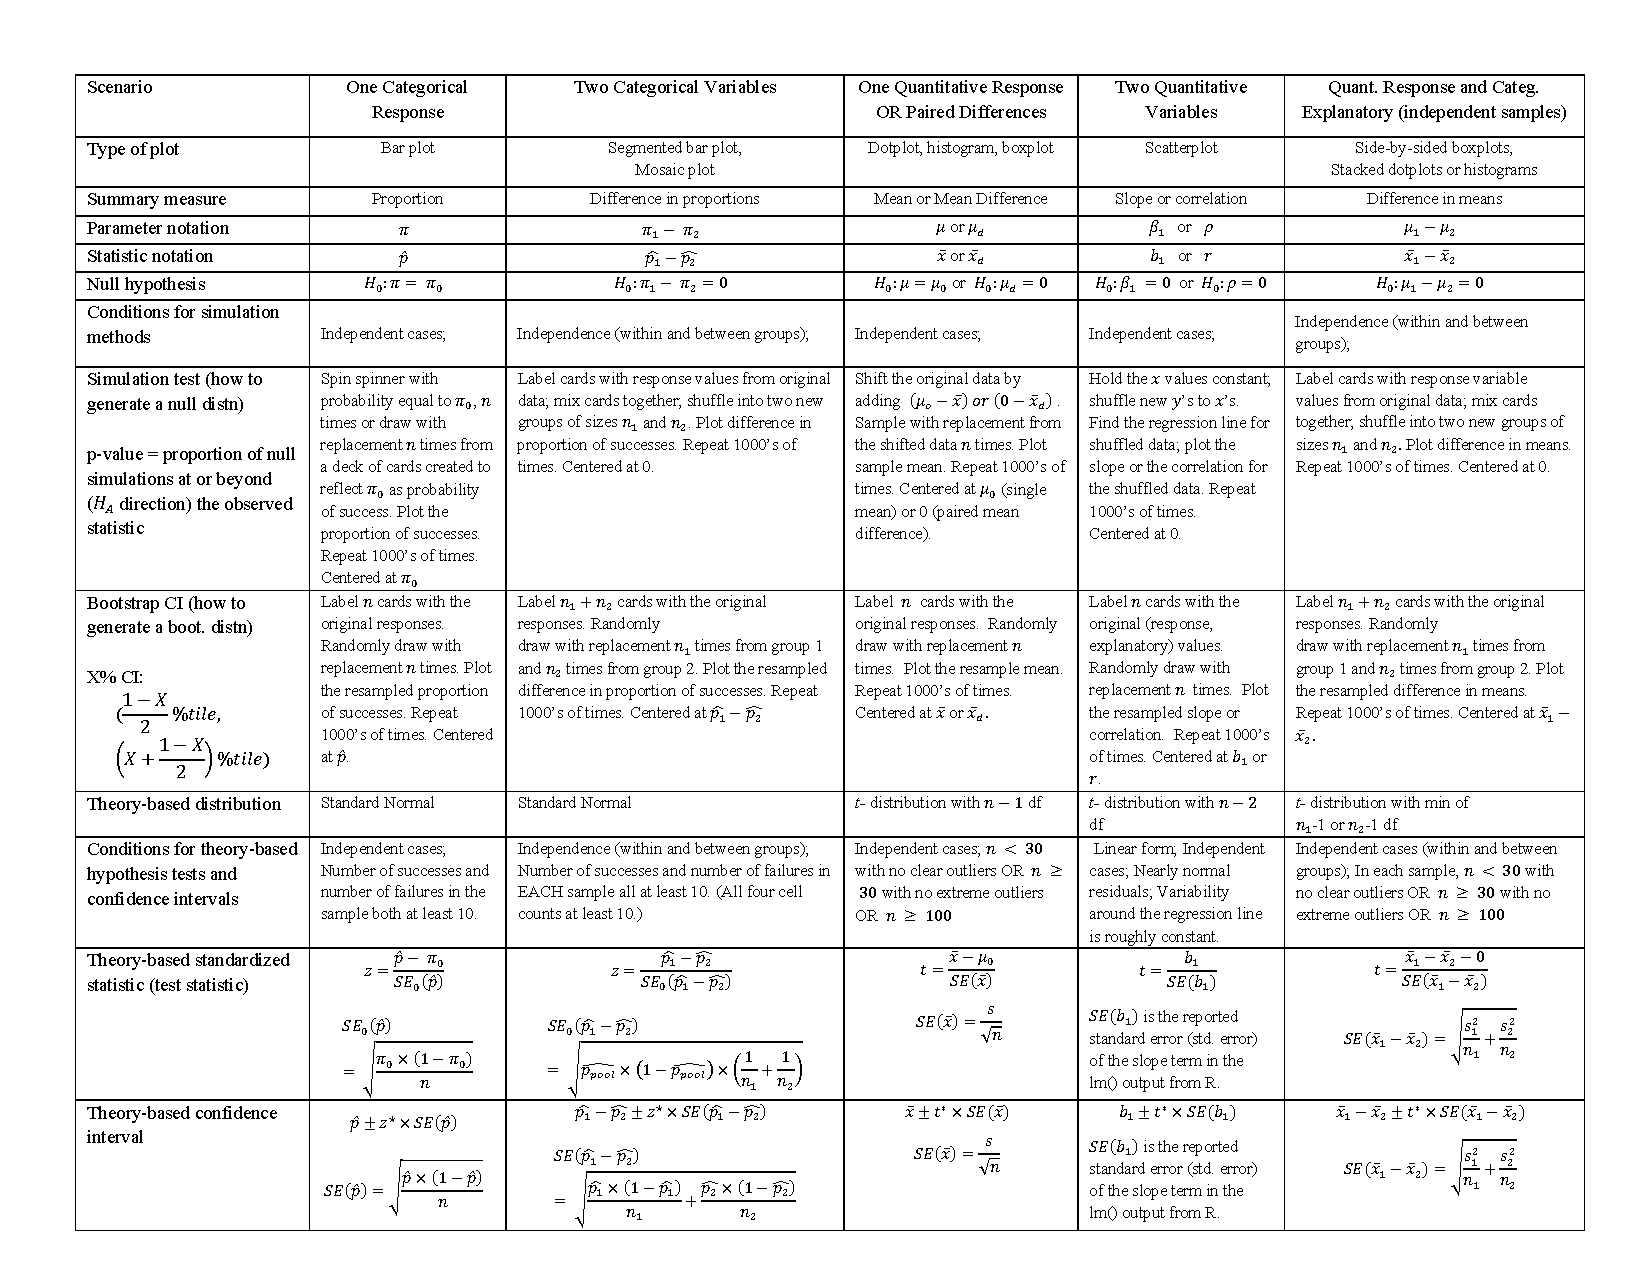
\includepdf[landscape=true]{GoldenTicket_F22.pdf}

\hypertarget{references}{%
\chapter*{References}\label{references}}
\addcontentsline{toc}{chapter}{References}

\hypertarget{refs}{}
\begin{CSLReferences}{1}{0}
\leavevmode\vadjust pre{\hypertarget{ref-pga}{}}%
{``Average Driving Distance and Fairway Accuracy.''} 2008. \href{https://www.pga.com/\%20and\%20https://www.lpga.com/}{https://www.pga.com/ and https://www.lpga.com/}.

\leavevmode\vadjust pre{\hypertarget{ref-islands}{}}%
Bulmer, M. n.d. {``Islands in Schools Project.''} \url{https://sites.google.com/site/islandsinschoolsprojectwebsite/home}.

\leavevmode\vadjust pre{\hypertarget{ref-darley1973}{}}%
Darley, J. M., and C. D. Batson. 1973. {``"From Jerusalem to Jericho": A Study of Situational and Dispositional Variables in Helping Behavior.''} \emph{Journal of Personality and Social Psychology} 27: 100--108.

\leavevmode\vadjust pre{\hypertarget{ref-ipeds}{}}%
Education Statistics, National Center for. 2018. {``IPEDS.''} \url{https://nces.ed.gov/ipeds/}.

\leavevmode\vadjust pre{\hypertarget{ref-zeitler2012}{}}%
Group, TODAY Study. 2012. {``\href{https://www.ncbi.nlm.nih.gov/pubmed/22540912}{A Clinical Trial to Maintain Glycemic Control in Youth with Type 2 Diabetes}.''} \emph{New England Journal of Medicine} 366: 2247--56.

\leavevmode\vadjust pre{\hypertarget{ref-hamblin2007}{}}%
Hamblin, J. K., K. Wynn, and P. Bloom. 2007. {``Social Evaluation by Preverbal Infants.''} \emph{Nature} 450 (6288): 557--59.

\leavevmode\vadjust pre{\hypertarget{ref-hirschfelder2018}{}}%
Hirschfelder, A., and P. F. Molin. 2018. {``I Is for Ignoble: Stereotyping Native Americans.''} \href{Retrieved\%20from\%20https://www.ferris.edu/HTMLS/news/jimcrow/native/homepage.htm.}{Retrieved from https://www.ferris.edu/HTMLS/news/jimcrow/native/homepage.htm.}

\leavevmode\vadjust pre{\hypertarget{ref-hutchison2013}{}}%
Hutchison, R. L., and M. A. Hirthler. 2013. {``\href{https://www.ncbi.nlm.nih.gov/pubmed/23932117}{Upper Extremity Injuies in Homer's Iliad}.''} \emph{Journal of Hand Surgery (American Volume)} 38: 1790--93.

\leavevmode\vadjust pre{\hypertarget{ref-imdb}{}}%
{``{IMDb} Movies Extensive Dataset.''} 2016. \url{https://kaggle.com/stefanoleone992/imdb-extensive-dataset}.

\leavevmode\vadjust pre{\hypertarget{ref-keating2021}{}}%
Keating, D., N. Ahmed, F. Nirappil, Stanley-Becker I., and L. Bernstein. 2021. {``Coronavirus Infections Dropping Where People Are Vaccinated, Rising Where They Are Not, Post Analysis Finds.''} \emph{Washington Post}. \url{https://www.washingtonpost.com/health/2021/06/14/covid-cases-vaccination-rates/}.

\leavevmode\vadjust pre{\hypertarget{ref-becentispeech}{}}%
Moquin, W., and C. Van Doren. 1973. {``Great Documents in American Indian History.''} Praeger.

\leavevmode\vadjust pre{\hypertarget{ref-weather}{}}%
National Weather Service Corporate Image Web Team. n.d. {``National Weather Service -- {NWS} Billings.''} \url{https://w2.weather.gov/climate/xmacis.php?wfo=byz}.

\leavevmode\vadjust pre{\hypertarget{ref-porath2017}{}}%
Porath, Erez, C. 2017. {``Does Rudeness Really Matter? The Effects of Rudeness on Task Performance and Helpfulness.''} \emph{Academy of Management Journal} 50.

\leavevmode\vadjust pre{\hypertarget{ref-quinn1999}{}}%
Quinn, G. E., C. H. Shin, M. G. Maguire, and R. A. Stone. 1999. {``Myopia and Ambient Lighting at Night.''} \emph{Nature} 399 (6732): 113--14. \url{https://doi.org/10.1038/20094}.

\leavevmode\vadjust pre{\hypertarget{ref-ramachandran2007}{}}%
Ramachandran, V. 2007. {``3 Clues to Understanding Your Brain.''} \url{https://www.ted.com/talks/vs_ramachandran_3_clues_to_understanding_your_brain}.

\leavevmode\vadjust pre{\hypertarget{ref-cdchospitalization}{}}%
{``Rates of Laboratory-Confimed COVID-19 Hospitalizations by Vaccination Status.''} 2021. CDC. \url{https://covid.cdc.gov/covid-data-tracker/\#covidnet-hospitalizations-vaccination}.

\leavevmode\vadjust pre{\hypertarget{ref-richardson2019}{}}%
Richardson, T., and R. T. Gilman. 2019. {``Left-Handedness Is Associated with Greater Fighting Success in Humans.''} \emph{Scientific Reports} 9 (1): 15402. \url{https://doi.org/10.1038/s41598-019-51975-3}.

\leavevmode\vadjust pre{\hypertarget{ref-stephens2020}{}}%
Stephens, R., and O. Robertson. 2020. {``Swearing as a Response to Pain: Assessing Hypoalgesic Effects of Novel "Swear" Words.''} \emph{Frontiers in Psychology} 11: 643--62.

\leavevmode\vadjust pre{\hypertarget{ref-stewart2014}{}}%
Stewart, E. H., B. Davis, B. L. Clemans-Taylor, B. Littenberg, C. A. Estrada, and R. M. Centor. 2014. {``Rapid Antigen Group a Streptococcus Test to Diagnose Pharyngitis: A Systematic Review and Meta-Analysis''} 9 (11). \url{https://doi.org/10.1371/journal.pone.0111727}.

\leavevmode\vadjust pre{\hypertarget{ref-stroop1935}{}}%
Stroop, J. R. 1935. {``Studies of Interference in Serial Verbal Reactions.''} \emph{Journal of Experimental Psychology} 18: 643--62.

\leavevmode\vadjust pre{\hypertarget{ref-sulheim2017}{}}%
Sulheim, S., A. Ekeland, I. Holme, and R. Bahr. 2017. {``Helmet Use and Risk of Head Injuries in Alpine Skiers and Snowboarders: Changes After an Interval of One Decade''} 51 (1): 44--50. \url{https://doi.org/10.1136/bjsports-2015-095798}.

\leavevmode\vadjust pre{\hypertarget{ref-titanic}{}}%
{``Titanic.''} n.d. \url{http://www.encyclopedia-titanica.org}.

\leavevmode\vadjust pre{\hypertarget{ref-covidvaccinetracker}{}}%
{``US COVID-19 Vaccine Tracker: See Your State's Progress.''} 2021. Mayo Clinic. \url{https://www.mayoclinic.org/coronavirus-covid-19/vaccine-tracker}.

\leavevmode\vadjust pre{\hypertarget{ref-usepa2020}{}}%
US Environmental Protection Agency. n.d. {``Air Data -- Daily Air Quality Tracker.''} \url{https://www.epa.gov/outdoor-air-quality-data/air-data-daily-air-quality-tracker}.

\leavevmode\vadjust pre{\hypertarget{ref-navajo2011}{}}%
{``Welcome to the Navajo Nation Government: Official Site of the Navajo Nation.''} 2011.\href{\%20Retrieved\%20from\%20https://www.navajo-nsn.gov/.}{Retrieved from https://www.navajo-nsn.gov/.}

\end{CSLReferences}

\end{document}
